\documentclass[11pt]{article}
\usepackage[utf8]{inputenc}
\usepackage[margin=1in]{geometry}
\usepackage[shortlabels]{enumitem}
\usepackage{bm}
\usepackage{amsfonts}
\usepackage{amssymb}
\usepackage{amsmath}
\usepackage{xcolor}
\usepackage{graphicx,caption}
\usepackage{amsthm}
\usepackage{qtree}
\usepackage{tree-dvips}
\usepackage{float}
\usepackage{authblk}
\usepackage{hyperref}
\usepackage{multirow}
\usepackage{algorithm2e}% http://ctan.org/pkg/algorithm2e
\makeatletter
\renewcommand{\@algocf@capt@plain}{above}% formerly {bottom}
\makeatother
\newtheorem{theorem}{Theorem}
\newtheorem*{theorem*}{Theorem}
\newtheorem{lemma}{Lemma}
\newtheorem*{lemma*}{Lemma}
\newtheorem{corollary}{Corollary}
\newtheorem*{corollary*}{Corollary}
\newtheorem{hypothesis}{Hypothesis}
\newtheorem*{hypothesis*}{Hypothesis}
\newtheorem{proposition}{Proposition}
\newtheorem{conjecture}{Conjecture}
\newtheorem{observation}{Observation}
\newtheorem{definition}{Definition}

\usepackage[numbers,sort&compress]{natbib}
\def\bibfont{\footnotesize}
\def\bibsep{\smallskipamount}
\def\bibhang{24pt}

\newcommand{\todo}[1]{\textcolor{red}{TODO: #1}}
\newcommand{\note}[1]{\textcolor{blue}{NOTE: #1}}
\newcommand{\dash}{\text{-}}
\newcommand{\B}{\{0,1\}}
\newcommand{\cat}{\mathbin\Vert}
\newcommand{\Jer}{Je\v{r}\'{a}bek }
\def\cl{\bf}
\author{Oliver Korten \thanks{Department of Computer Science, Columbia University. Email: \href{mailto:oliver.korten@columbia.edu}{oliver.korten@columbia.edu}}}
\date{}
\title{Derandomization from Time-Space Tradeoffs}
\begin{document}
\maketitle
\begin{abstract}
A recurring challenge in the theory of pseudorandomness and circuit complexity is the explicit construction of ``incompressible strings,'' i.e. finite objects which lack a specific type of structure or simplicity. In most cases, there is an associated {\cl NP} search problem which we call the ``compression problem,'' where we are given a candidate object and must either find a compressed/structured representation of it or determine that none exist. For a particular notion of compressibility, a natural question is whether an efficient algorithm for the compression problem would aide us in the construction of incompressible objects. Consider the following two instances of this question:
\begin{enumerate}
    \item Does an efficient algorithm for circuit minimization imply efficient constructions of hard truth tables?
    \item Does an efficient algorithm for factoring integers imply efficient constructions of large prime numbers?
\end{enumerate} 
In this work, we connect these kinds of questions to the long-standing challenge of proving time-space tradeoffs for Turing machines, and proving stronger separations between the RAM and 1-tape computation models. In particular, one of our main theorems shows that modest time-space tradeoffs for deterministic exponential time, or separations between basic Turing machine memory models, would imply a positive answer to both (1) and (2). 
These results apply to the derandomization of a wider class of explicit construction problems, where we have some efficient compression scheme that encodes $n$-bit strings using $<n$ bits, and we aim to construct an $n$-bit string which cannot be recovered from its encoding.
\end{abstract}
\newpage
\section{Introduction}\label{sec:intro}
Mathematicians have long been familiar with the curious phenomenon of a \emph{non-constructive proof}: an argument which demonstrates the existence of an object satisfying some special property, but which fails to indicate a particular example of such an object.
The advent of complexity theory has provided us with a formal way of defining the level of ``inherent constructivity'' in a theorem: we can say that an existence theorem is constructive if there is an accompanying polynomial time algorithm supplying an example of one of the objects the theorem proves to exist, and is inherently non-constructive if no such algorithm exists. Papadimitriou initiated a formal complexity-theoretic treatment of this topic three decades ago \cite{christos}, where he provided a taxonomy of total search problems (problems that always have solutions) in {\cl NP} by classifying them based on the strength of the lemma guaranteeing the existence of a solution on all instances.

When a particular theorem appears to be inherently non-constructive, in that no polynomial time algorithm can witness the solutions it guarantees, one perspective we can take is that this theorem is ``effectively false'' in a certain context, despite being irrefutably true in general. This is essentially the outlook presented by Yao in his seminal paper introducing the basis of theoretical cryptography \cite{Yao}. Here, Yao focuses on the central tenets of Shannon's information theory.
He argues that although Shannon's theorems are of course provably correct, in many scenarios it appears computationally infeasible to witness their truth. For example, an output of some function $f \colon\B^n \rightarrow \B^{2n}$ under the uniform distribution on $\B^n$ has entropy $n$, and thus by a result of Shannon can be encoded on average using $n$ bits. However for an observer who sees only the outputs of this distribution, there seems to be no efficient way to generate such a code without the ability to efficiently invert $f$. If we posit that there are some specific functions $f$ for which it is in fact impossible to efficiently realize Shannon's theorem in this sense, one might venture to say that Shannon's theorem \emph{effectively fails} for $f$ in the computational realm, perhaps allowing us to carry out tasks which would, in the absence of computational constraints, be deemed impossible. Indeed it is widely conjectured that there are efficiently computable functions $f$ of this form, and this conjecture underpins the security of many cryptographic protocols. Similar situations are abundant in the field of cryptography, where the computational infeasibility of \emph{witnessing} impossibility theorems from information theory allows us to effectively bypass them.

With this perspective in mind, let us now turn our attention to a special family of non-constructive proofs of great interest to complexity theorists, proofs which guarantee the existence of ``pseudorandom objects.'' Key examples include the existence of truth tables of high circuit complexity and of pseudorandom generators capable of derandomizing algorithms. The task of making these proofs constructive is often referred to as an ``explicit construction problem,'' since the goal is to print one explicit example of an object possessing some pseudorandom property. In \cite{Korten} it is shown that a broad collection of such problems can be reduced to the following more general task: given some efficiently computable function $f\colon \B^{n-1} \rightarrow \B^n$, find an $n$-bit string outside the range of $f$. The existence of a solution is guaranteed by the ``dual weak pigeonhole principle,'' and indeed this principle guarantees that a \emph{randomly chosen} string is a solution with high probability. The question at hand is whether this principle is \emph{inherently nonconstructive}. Unlike the case of Shannon's theorems on information transmission, the prevailing wisdom in complexity theory is this theorem \emph{can be made constructive}: it is widely conjectured that exponential time requires exponential circuit size, and by \cite{Korten}, this would in fact imply a generic non-trivial\footnote{The implied witnessing algorithm runs in ${\cl P}^{\cl NP}$, whereas the trivial upper bound for this problem is ${\cl \Sigma_2^P}$.} ``witnessing'' algorithm for the dual weak pigeonhole principle, i.e. an algorithm which produces $n$-bit strings outside the range of any such $f$. 

In search of evidence for this widely-conjectured belief that the weak pigeonhole principle can be made more constructive, the starting point of this work is to imagine what the computational landscape would look like if it were false, i.e. if we lived in a world where there was an ``effective counterexample'' to the weak pigeonhole principle. In particular, let us model this scenario by supposing that there are a pair of efficiently computable functions  $\mathcal{G} = \{g_n \colon \B^{n} \rightarrow \B^{n-1}\}_{n \in \mathbb{N}}$, $\mathcal{F} = \{f_n \colon \B^{n-1} \rightarrow \B^n\}_{n \in \mathbb{N}}$, such that no polynomial time algorithm is able to construct an $n$-bit string $x$ such that $f_n(g_n(x)) \neq x$ in $poly(n)$ time (for more then finitely many $n$). Note that this is a slightly different version of the weak pigeonhole principle then what we defined in the previous paragraph: here we are given both the length-increasing function $f$ and a supposed inverse $g$, and the pigeonhole principle tells us that $f \circ g$ cannot be the identity.
% For this problem, widely-conjectured circuit lower bounds would imply a polynomial time deterministic witnessing algorithm. 
In this hypothetical world where $\mathcal{F}, \mathcal{G}$ are an ``effective counterexample'' to the weak pigeonhole principle, we have access to an efficient compression scheme which allows us to encode any $n$-bit string using $n-1$ bits. What improbable feats can be accomplished in such a world? 

In this work we give one answer to this question: if the weak pigeonhole principle \emph{effectively fails} in the above sense, we can utilize this failure to construct an efficient data structure which allows us to simulate RAM computations in low space and near-linear time on a 1-tape Turing machine.
Stated in contrapositive, mild time-space tradeoffs for simulating RAM machines on a 1-tape Turing machine would imply a generic algorithm to witness the weak pigeonhole principle, and in turn would have significant consequences in the theory of pseudorandomness and circuit complexity. 

% We also make progress towards a characterization of \emph{full derandomization} (i.e. ${\cl prBPP} = {\cl prP}$) in terms of total search problems, by demonstrating a total search problem related to the weak pigeonhole principle which is compete for {\cl prBPP} under deterministic reductions. While the arguments underlying this proof are decades-old and completely standard, \todo{it's a nice way of looking at things...}. In the course of this proof, we observe that if a particular step in Yao's hybrid argument can be derandomized, then every problem in ${\cl prBPP}$ reduces to a search problem in ${\cl PPP} \subseteq {\cl TFNP}$.
\subsection{Our Contributions}\label{subsec:contr}
\subsubsection{Derandomization from Time-Space Tradeoffs}
Let $\mathcal{C}, \mathcal{D} = \{C_n\colon \B^{n} \rightarrow \B^{n-1}\}_{n \in \mathbb{N}}, \{D_n\colon \B^{n-1} \rightarrow \B^{n}\}_{n \in \mathbb{N}}$. We call such a pair a ``uniform compression scheme,'' where $\mathcal{C}$ is the ``compressor'' which encodes $n$-bit ``messages'' by $n-1$-bit ``codewords,'' and $\mathcal{D}$ is the ``decompressor'' which maps $n-1$-bit codewords to the messages they represent\footnote{The formal definition given in Section~\ref{sec:pigeons} is slightly more general, but we will focus on this special case for now.}. We use the term ``uniform'' since in the relevant cases, $\mathcal{C}$ and $\mathcal{D}$ will each be described by a single Turing machine which computes $C_n$ (resp. $D_n$) for all $n$. We will say that a string $x \in \B^n$ is ``incompressible'' for such a scheme if $D_n(C_n(x)) \neq x$, i.e. if $\mathcal{D}$ cannot be used to recover the message $x$ from the codeword assigned to it by $\mathcal{C}$. In this paper, we study the complexity of the \emph{explicit construction task} of generating incompressible strings for uniform compression schemes. This task can be viewed naturally as a derandomization problem, since a randomly chosen $n$-bit string will be incompressible with high probability with respect to any fixed compression scheme.

Our results then show how to derive efficient derandomized algorithms for generating incompressible strings, assuming certain \emph{uniform} lower bounds. The lower bounds we consider are time-space tradeoffs for simulating RAM by 1-tape machines. Roughly, they posit that there are problems solvable in time $T$ on a RAM machine which cannot be solved on a 1-tape machine using $T^{0.01}$ space and $T^{1.01}$ time. Depending on certain features of the compression scheme and the resources available to the explicit construction algorithm, the specifics of the tradeoff assumption will vary, as we shall explain in Figure~\ref{fig:results}.

Initially, we consider the case of ``poly-time compression schemes'', where both $\mathcal{C}$ and $\mathcal{D}$ are computable in polynomial time. We show that for such schemes, incompressible strings can be constructed deterministically in polynomial time assuming time-space tradeoffs for deterministic exponential time:
\begin{theorem*}[Theorem~\ref{thm:tisp-impl}]
Suppose there is some exponential time bound $T(n) \geq 2^{\Omega(n)}$ and some $\epsilon > 0$ such that it is impossible to simulate $T(n)$-time RAM computations on 1-tape Turing machines that use $T(n)^{1+\epsilon}$ time and $T(n)^{\epsilon}$ space. Then for any poly-time compression scheme, there is a polynomial time algorithm that produces incompressible $n$-bit strings for this scheme on input $1^n$ (for infinitely many $n$).
\end{theorem*}


Constructing incompressible strings for poly-time compression schemes is a natural and quite broad derandomization problem. Theorem~\ref{thm:tisp-impl} gives a novel connection between derandomizing this task and proving \emph{uniform} time-space tradeoffs-- in contrast, the assumptions previously required to derandomize this sort of problem require a lower bound against \emph{non-uniform} algorithms, such as circuits. To put this derandomization task in a more familiar context, in Section~\ref{subsec:particular-pairs} we show that several well-studied explicit construction problems, such as the construction of large prime numbers or the construction of truth tables of high circuit complexity/formula size, can be reduced to the problem of finding incompressible strings for some uniform compression scheme. In each case, the compression scheme will either be computable efficiently, or efficiently with access to an oracle for some search problem in {\cl FNP} which is not known to be {\cl NP}-complete. 
% We then consider, for some compression scheme $\mathcal{C},\mathcal{D}$, whether there is an efficient explicit construction algorithm that produces incompressible strings for the scheme. Our main results show that if there is no such algorithm, this implies the existence of a highly effective simulation of RAM machines using low space on a 1-tape machine, which makes short oracle queries to $\mathcal{C}, \mathcal{D}$. Depending on the precise features of the explicit construction algorithm presumed not to exist, our simulation will have varying properties. Ultimately these results are most interesting when stated in contrapositive form: they show that, assuming basic tradeoffs between time and space are necessary when converting a RAM algorithm to a 1-tape algorithm, a range of explicit construction problems can be efficiently derandomized.\\

To state our other main results in their most interesting form, we focus our attention now on the construction of strings/truth tables of high complexity with respect to some non-uniform complexity measure, such as formula size, circuit size, or time-bounded Kolmogorov complexity. In each case there is an associated {\cl NP} search problem, where we are given a string/truth table and must find a small formula/circuit/program computing it (if one exists); we call this the ``compression problem.'' The following table shows how our three main theorems relate various time-space tradeoff hypotheses to such problems:

\begin{figure}[H]
    \centering
    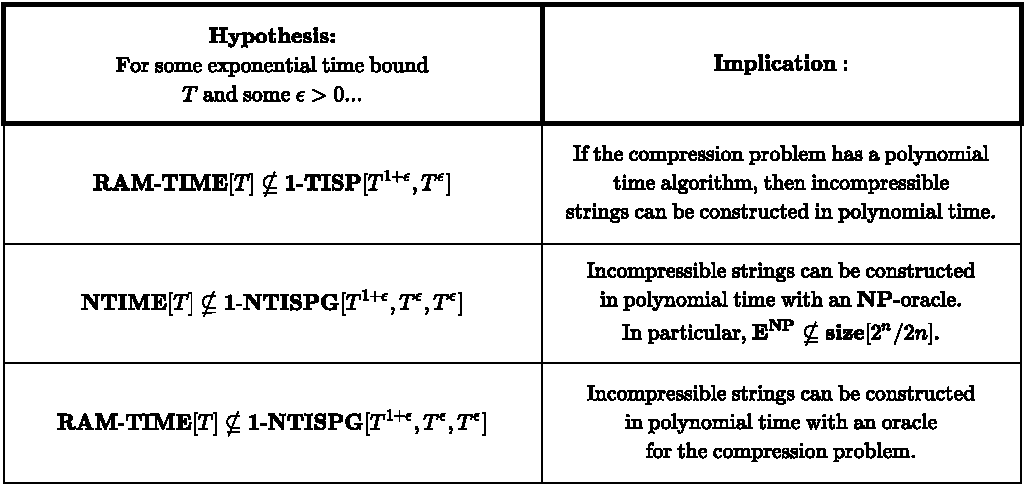
\includegraphics[width=1\textwidth]{space_results_table.pdf}
    \caption{Main Results. We use the shorthand $T=T(n)$.}
    \label{fig:results}
\end{figure}

The classes seen on the left hand side will be defined formally in Section~\ref{subsec:machines}, but we give a brief explanation here so that the table can be interpreted appropriately. ${\cl TIME}[T(n)]$ and ${\cl NTIME}[T(n)]$ are defined in the standard way using multitape machines; the prefixes ${\cl 1}$ and ${\cl RAM}$ indicate, respectively, either a restriction of the model to 1-tape machines or a strengthening to random access machines. The class ${\cl TISP}[T(n),S(n)]$ consists of problems decidable simultaneously in time $T(n)$ and space $S(n)$. Finally, ${\cl NTISPG}[T(n),S(n),G(n)]$ consists of problems decidable by a nondeterministic machine running in time $T(n)$ which, on every computation path, uses at most $S(n)$ space and $G(n)$ nondeterministic guesses.

For a concrete example of how to apply these results, lets focus on the compression problem {\sc Circuit Synthesis} (given a truth table find a small circuit for it if one exists), and the explicit construction problem of producing truth tables of exponential circuit complexity. The first hypothesis in the above table implies that if {\sc Circuit Syntheses} is in {\cl P} then there is a polynomial time construction of hard truth tables (i.e. ${\cl E}$ has exponential circuit complexity). The second hypothesis implies unconditionally that there is an efficient ${\cl NP}$ oracle construction of hard truth tables (i.e. ${\cl E}^{\cl NP}$ has exponential circuit complexity). Finally, the third and strongest hypothesis tells us that there is a polynomial time construction of hard truth tables using an oracle for {\sc Circuit Synthesis}.
\\
\\
The case of large prime construction does not fit in as neatly to the above picture, as the scheme we devise for this problem will require a factoring oracle for both the compressor and decompressor (while the above problems have a polynomial-time computable decompressor). In this case we get the following result:
\begin{theorem*}[Corollary~\ref{cor:prime-construction}]
Under the hypothesis in the top row of the above table, a polynomial time algorithm for factoring implies a polynomial time algorithm to construct $32n$-bit primes of magnitude $>2^n$ for infinitely many $n$.
\end{theorem*}

If we forgo the questionable assumption that factoring lies in {\cl P}, we get:
\begin{theorem*}[Corollary~\ref{cor:factoring-oracle}]
One of the following is true:
\begin{enumerate}
    \item For every exponential time bound $T$ and every $\epsilon>0$, every language decidable in time $T(n)$ on a RAM machine can be decided in time $T(n)^{1+\epsilon}$ and space $T(n)^{\epsilon}$ by a 1-tape machine with a factoring oracle, which makes oracle calls of length at most $T(n)^{\epsilon}$.
    \item There is a polynomial time algorithm with a factoring oracle that generates $32n$-bit primes of magnitude $>2^n$ for infinitely many $n$.
\end{enumerate}
\end{theorem*}

The problem of deterministically generating large primes has been investigated previously in several works, and was notably the subject of the Polymath 4 project \cite{polymath}. In the public discussion forums for this project, it was explicitly asked whether a polyomial time algorithm for factoring, or more generally an oracle for factoring, would help. More recently, Oliviera and Santhanam gave a subexponential time ``pseudodeterministic'' construction of large primes \cite{pseudo-primes}, using only the fact that primality is testable in {\cl P} \cite{primes} and that primes occur with non-negligible frequency.

\subsubsection{BPP and the Weak Pigeonhole Principle}
In Section~\ref{sec:bpp} we briefly consider the relationship between various search problems associated with the weak pigeonhole principle, and the ``full derandomization task'' characterized by the class {\cl prBPP}. Observe that the problem introduced above of finding incompressibe strings for uniform compression schemes can be generalized to a {\cl TFNP} search problem -- instead of considering compression schemes generated by uniform Turing machines, we can consider the search problem where a compression scheme of some fixed length is given as input in the form of a pair of boolean circuits:
\begin{definition}
In {\sc Lossy Code}, we are given as input a pair of circuits $C\colon \B^n \to \B^{n-1}$, $D\colon\B^{n-1}\to\B^n$, and must output some $x \in \B^n$ such that $D(C(x))\neq x$.
\end{definition}

While finding a deterministic algorithm for {\sc Lossy Code} appears to be a quite generic derandomization problem, it would be a major breakthrough to show that {\sc Lossy Code} captures the ``full derandomization problem:'' since {\sc Lossy Code} lies in {\cl TFNP}, if {\cl prBPP} reduces to {\sc Lossy Code} then ${\cl BPP} \subseteq {\cl NP}$, which is a notorious open problem. In Section~\ref{sec:bpp}, we show that a natural generalization of {\sc Lossy Code}, where we allow the compressor $C$ to be randomized, is indeed strong enough to characterize {\cl prBPP} precisely. The formal problem is as follows:
\begin{definition}
In {\sc R-Lossy Code}, we are given as input circuits $C\colon \B^n \times \B^m \to \B^{n-1}$, $D\colon \B^{n-1}\to\B^n$, and must find some $x$ such that $Pr_r [D(C(x,r))=x] < \frac{1}{2}$. 
\end{definition}
In this work we demonstrate:
\begin{theorem*}[Theorem~\ref{thm:bpp-pigeon}]
{\sc R-Lossy Code} is complete for {\cl prBPP} under deterministic Turing reductions.
\end{theorem*}

The relation between pigeonhole principle search problems and more standard derandomization problems is summarized in Figure~\ref{fig:bpp}. 
\begin{figure}[ht]
    \centering
    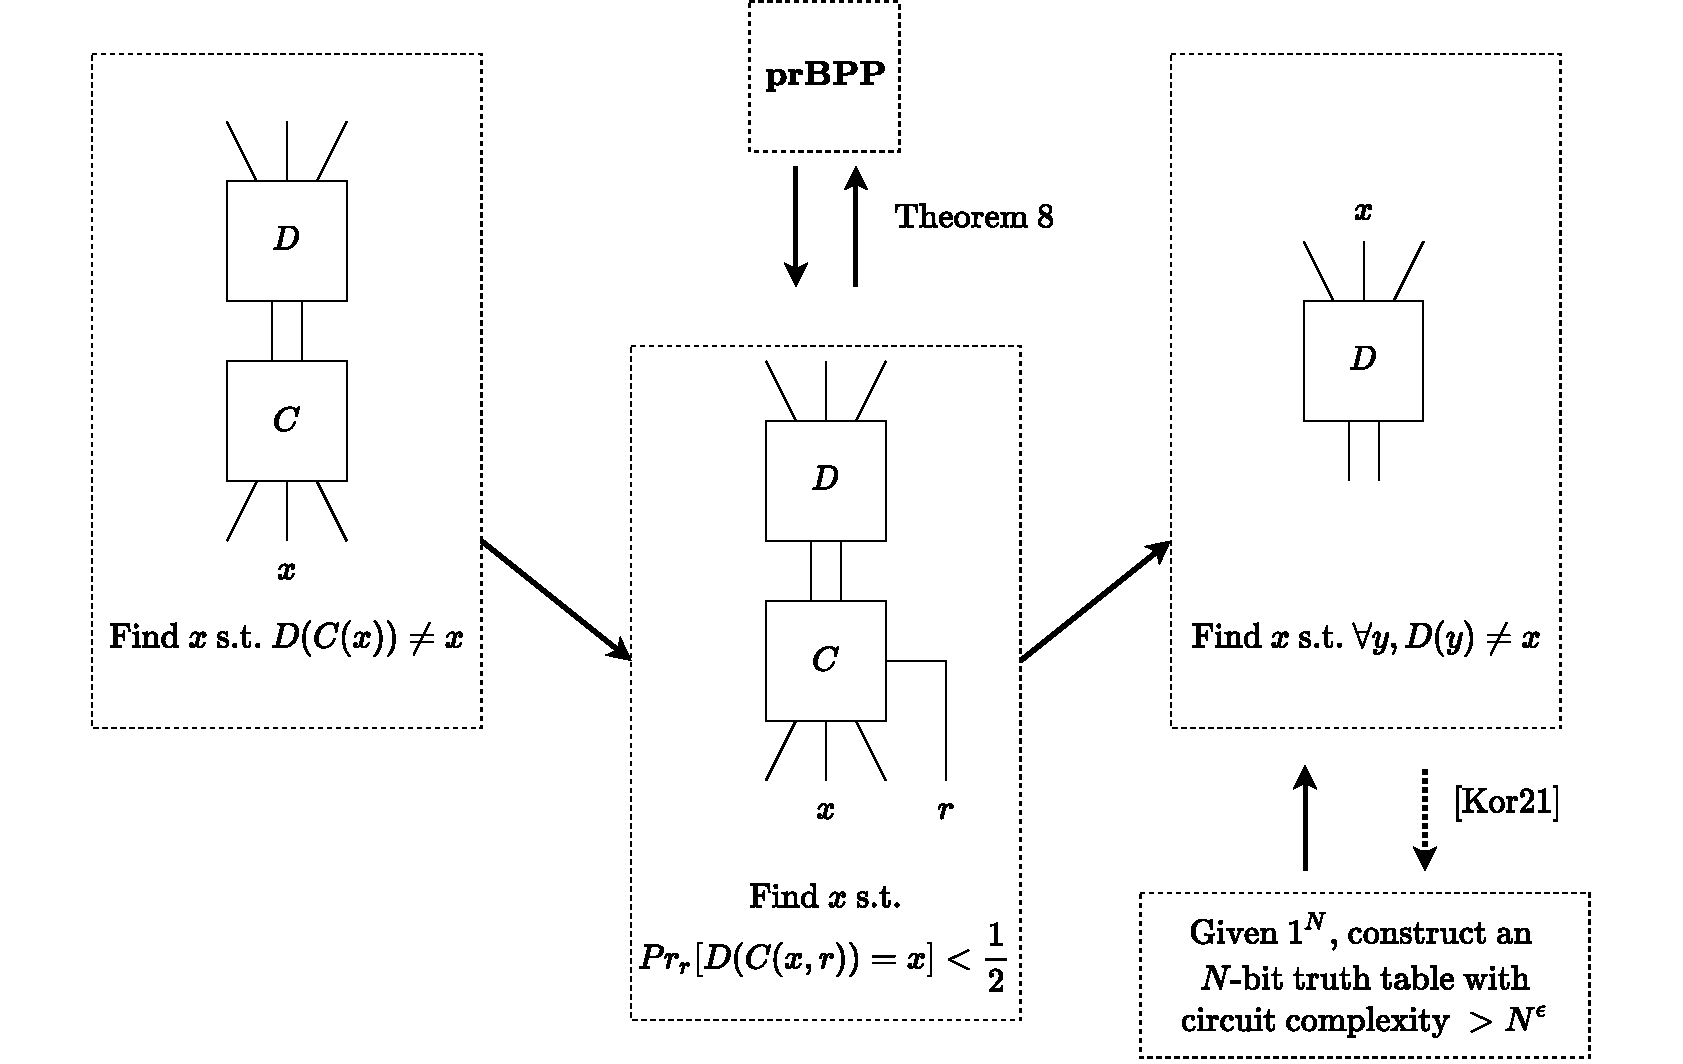
\includegraphics[width=0.8\textwidth]{php_bpp_picture.pdf}
    \captionsetup{width=1\textwidth}
    \caption{Relations between the total search problems associated with various weak pigeonhole principles, and standard derandomization problems. Solid arrows represent deterministic polynomial time reductions, while dotted arrows represent {\cl NP}-oracle reductions.}
    \label{fig:bpp}
\end{figure}

The proof of Theorem~\ref{thm:bpp-pigeon} is mostly standard, following quite directly from Yao's next bit predictor lemma. From the proof of this theorem we are able to extract the following interesting corollary:
\begin{corollary*}[Corollary~\ref{cor:yao}, Informal]
If the fixing of the leftover bits in Yao's hybrid argument can be derandomized, then ${\cl BPP} \subseteq {\cl NP}$. Indeed, under this assumption, every problem in ${\cl prBPP}$ reduces to the search problem {\sc Lossy Code} in ${\cl PPP} \subseteq {\cl TFNP}$.
\end{corollary*}

In other words, derandomizing a particular step in Yao's classical argument implies a quite universal derandomization of {\cl prBPP}.
\subsection{Relation to Prior Work}\label{subsec:prior}
\paragraph{Hardness vs. Randomness}
As mentioned above, the task of constructing incompressible strings can be naturally viewed as a derandomization problem, and is thus amenable to the standard hardness/randomness paradigm. In particular, when the compression scheme is polynomial time computable as in Theorem~\ref{thm:tisp-impl}, the standard hardness assumptions used to derandomize {\cl BPP} (e.g. \cite{IW}) would suffice to yield a polynomial time construction of incompressible strings. Such hardness assumptions require a lower bound for a language in {\cl E} against some non-uniform model of computation, such as boolean circuits. In contrast, Theorem~\ref{thm:tisp-impl} gives a hardness/randomness connection for this problem which only requires a \emph{uniform lower bound} for a a language in {\cl E}, in particular a lower bound against low-space algorithms running in slightly more time using a weaker memory model.
% \paragraph{Karp-Lipton Theorems:} 
% As \todo{somethin}, the existence of explicit construction  algorithms witnessing the weak pigeonhole principle is intimately connected to the circuit complexity of exponential time classes. Since our results prove the existence of such algorithms assuming certain time-space lower bounds for uniform classes, these results can be broadly placed within the framework of ``Karp-Lipton type theorems:'' theorems which derive non-uniform circuit lower bounds from separations between uniform classes \cite{karp-lipton}. Perhaps most relevant are the collapses due to Meyer \cite{karp-lipton} and to Babai, Fortnow and Lund \cite{BFL}, which show that for various exponential time classes such as ${\cl EXP}, {\cl NEXP}$, or ${\cl EXP}^{\cl NP}$, if these classes have small circuits then they in fact collapse to low levels of the polynomial hierarchy, and in particular must lie in {\cl PSPACE}. When scaled upwards appropriately, these results would imply that, unless there are explicit constructions of truth tables with exponential circuit complexity, ${\cl E}$ can be decided in $2^{\epsilon n}$ space for any $\epsilon > 0$. Stated contrapositively, this means that if ${\cl E}$ \emph{cannot} be solved in subexponential space, then circuit lower bounds (and thus a constructive proof of the pigeonhole principle) follow. At the surface this seems roughly similar to the results we obtained above. However, the simulation implied by these results would have time complexity roughly $2^{2^{\epsilon n}}$, which is far less efficient then what we show above. In this sense, the uniform separations that we assume are much weaker then what is required to apply known Karp-Lipton style theorems: we leave open the possibility that exponential time can be simulated in very low (even polynomial space), but simply posit that such a simulation would require a strongly superlinear blowup in time.

\paragraph{The Easy Witness Lemma:} Perhaps the closest prior work to our results is the ``Easy Witness Method,'' initiated by \cite{Kabenets} and furthered in \cite{IKW} and \cite{williams-sat}, which roughly says that assuming ${\cl E}^{\cl NP}$ has small circuits, any nondeterministic exponential time computation must have witnesses of low circuit complexity. This immediately implies that unless ${\cl E}^{\cl NP}$ requires large circuits, we can efficiently simulate ${\cl NTIME}[2^n]$ using limited nondeterminism by ``guessing a small circuit.'' In Appendix~\ref{appendix:ewl}, we show that this old method (along with one other well-known tool) is in fact enough to prove the second implication in Figure~\ref{fig:results}, although this connection to time-space tradeoffs does not seem to have been noted previously. However, this proof heavily utilizes the distinctive power of nondeterminism, whereby additional ``guesses'' allow us to vastly simplify the verification procedure, and does not seem to extend to our other two main results.

\subsection{Known Time-Space tradeoffs:}\label{subsec:known-tradeoffs}
Finally, we cover the known results on time-space tradeoffs and separations between the RAM and 1-tape models. We first emphasize the following: all three time-space tradeoff hypotheses stated on the left-hand side of Figure~\ref{fig:results} are known to hold \emph{unconditionally} when the time bound $T$ is $O(n)$. In particular, an old result of Maass \cite{palindromes} shows that the set of palindromes is recognizable in quasilinear time on a deterministic RAM machine, but requires $\Omega(n^2)$ time on a nondeterministic 1-tape machine. However, Maass's proof is essentially a counting argument which crucially relies on the entropy of the input being comparable in magnitude to the total computation time, which is no longer the case for exponential time computations. When it comes to separating the RAM and 1-tape models for generic time bounds, a result of \cite{robson} shows that there must be \emph{some} slowdown when simulating a RAM on a 1-tape machine for \emph{any time bound} greater then $n \log \log n$, but the slow-down is an astronomically small multiplicative factor, on the order of $\log \log T(n)$. 

Another sequence of works (\cite{fortnow}, \cite{tisp-sat}, \cite{williams-tisp} among others) has shown unconditionally that nondeterministic linear time cannot be solved in ${\cl TISP}[n^{1+\epsilon}, n^{\epsilon}]$ for certain fixed values of $\epsilon>0$, even when the simulating machine is given access to RAM. These results can be scaled to larger time bounds as follows: for any time-constructible $T$, ${\cl \Sigma_2 TIME}[T(n)]$ is not contained in ${\cl TISP}[T(n)^{1+\epsilon}, T(n)^{\epsilon}]$ for certain fixed values of $\epsilon>0$. Such results are obtained by combining hierarchy theorems with a fast simulation result, whereby a ${\cl \Sigma_2}$ machine can simulate a ${\cl TISP}[T(n)^{1+\epsilon}, T(n)^{\epsilon}]$ computation in time $T(n)^{1 - \delta}$ time for some fixed $\epsilon, \delta > 0$. It is evident that such results will not be sufficient for our purposes, as they only rule out efficient low-space simulations of ${\cl \Sigma_2}$ computations by deterministic machines.


\subsection{Main Tool: the J-tree}
The basis of our main proofs is a construction which we call the ``J-tree.'' Roughly speaking, the J-tree is a data structure which allows us to store an array of $T$ elements, subject to fast update/query operations, using significantly less then $T$ bits. While this task is information-theoretically impossible (by the weak pigeonhole principle), the J-tree uses a compression scheme $C,D$ to perform its operations, and whenever it fails in its role as a data structure, it is able to print out an incompressible string for this scheme. Thus, assuming no polynomial time algorithm can witness the weak pigeonhole principle for $C,D$, no polynomial time algorithm can witness the failure of this data structure. This will allow our low-space simulations to operate a RAM memory using low space on a 1-tape machine, in such a way that if the simulation fails, then a polynomial time algorithm can witness this failure, and thus witness the weak pigeonhole principle for $C,D$.

The core construction underlying the J-tree has an intriguing history dating back to the late 1970's. In the course of a decade, this construction was used, seemingly independently, to prove three seminal results in cryptography and logic: 
\begin{enumerate}
    \item In 1979\footnote{Although the cited work is dated to 1988, Merkle filed a patent for the concept about a decade earlier.}, Merkle showed how to iterate a cryptographically secure hash function $h\colon \B^{2n} \rightarrow \B^n$ in a tree-like fashion to construct a secure digital signature scheme whose signature size increases logarithmically in the number of messaged signed \cite{Merkle}\footnote{The Merkle Tree is in some sense ``dual'' to the other two examples, as it iterates a function which \emph{compresses} strings by a factor of two, while the others iterate a function that \emph{extends} by a factor of two.}.
    \item In 1986, Goldwasser Goldreich and Micali showed how to iterate a pseudorandom generator $G\colon \B^n \rightarrow \B^{2n}$ in a similar tree-like manner into a family of functions $\{G_x\colon \B^n \rightarrow \B^n\}_{x \in \B^n}$ whose input/output behaviours are indistinguishable from random, assuming $G$ is a secure PRG \cite{GGM}.
    \item In 1988, Paris, Wilkie, and Woods gave a novel proof of the weak pigeonhole principle in bounded arithmetic\cite{Paris-Wilkie-Woods}. Again, the same process of iterating a function $f\colon \B^n \rightarrow \B^{2n}$ is applied. Here, the function $f$ is assumed to be a bijection between $\B^n$ and $\B^{2n}$, and the iteration procedure is the first step towards establishing a contradiction in the relevant proof system.
\end{enumerate}

Following \cite{Paris-Wilkie-Woods}, \Jer \cite{Jerabek} used this same construction within bounded arithmetic to establish a deep connection between the weak pigeonhole principle and circuit complexity. This work most closely informs our perspective, hence the name ``J-tree.'' In \cite{Korten}, the techniques of \Jer were translated to the language of traditional complexity theory, which yield the following interpretation of this tree-like iteration process: given a circuit $D\colon \B^n \rightarrow \B^{2n}$, we can efficiently construct a new circuit $D^*\colon \B^n \rightarrow \B^{2^k n}$ satisfying the following: any string in the range of $D^*$ is a truth table of low circuit complexity, and any string outside the range of $D^*$ can be used to efficiently construct a string outside the range of $D$ using an {\cl NP} oracle. If we have a compression scheme $C\colon\B^{2n}\rightarrow \B^n, D\colon\B^n\rightarrow \B^{2n}$, the same argument lets us iterate these to a scheme $C^*,D^*$ of message length $2^kn$ and code length $n$, where again $D^*$ always outputs low complexity truth tables, and now we have that any incompressible string for $C^*,D^*$ can be transformed in polynomial time (without an oracle) into an incompressible string for $C,D$.

Thus, if it is hard to witness the weak pigeonhole principle for $C,D$, then we will be able to take any string (``message'') of length $2^kn$ and find a small circuit computing it (``codeword'') by feeding it through $C^*$. A circuit can naturally be interpreted as a data structure storing an array subject to fast query operations: the truth table represents the contents of the array, and the circuit allows us to efficiently compute a particular bit in the truth table given its index. However, to use the J-tree to simulate RAM computations, we will also require fast update operations, which let  us set a position in the array to a new value. Our main addition to this line of work is the ``J-Tree Update Lemma'' (Lemma~\ref{lem:updates}), which gives a procedure that accomplishes this second task. The Update Lemma does not seem to have an analogue in any of the previously mentioned works.
\section{Preliminaries}\label{sec:prelim}
\subsection{Basics}\label{subsec:basics}
Our notation for basic concepts is standard, e.g. all logarithms are base 2, we use $[n]$ to denote $\{1,\ldots,n\}$, $|x|$ to denote length of a binary string. We will define the following precise notion of an ``exponential time bound:''
\begin{definition}
We say a function $T\colon \mathbb{N} \rightarrow \mathbb{N}$ is an ``exponential time bound'' if $T$ is time constructible, and there exist constants $0< \beta < B$ such that for sufficiently large $n$, $2^{\beta n} \leq T(n) \leq 2^{Bn}$.
\end{definition}
This is in contrast to the more general notion of exponential growth where we have $2^{n^\beta} \leq T(n) \leq 2^{n^B}$. 

\subsection{Machine Models}\label{subsec:machines}
We start by precisely defining the various machine models and complexity classes that will be used. We begin with a definition of ``random access memory'' or ``RAM'' machines:
\begin{definition}[RAM machines]
A RAM machine is a turing machine equipped with two binary tapes, one called the ``auxilliary tape'' and the other called the ``addressing tape.'' We collectively refer to these as the ``linear tapes.'' Both linear tapes admit the same operations as a standard Turing machine tape, where in one step we can move the head left/right and read or modify a cell of the tape. In addition, there is an associated ``RAM memory'' consisting of a sequence of binary variables $A_1,A_2,\ldots$. The addressing tape has two additional operations that allow it to interact with the RAM memory. There is an $\mathsf{Update}$ operation, which in one step sets $A_i = b$, where $i$ is the integer whose binary representation lies to the left of the addressing tapehead, and $b$ is the bit currently read by the auxiliary tape. There is also a $\mathsf{Load}$ operation, which in one step sets the cell pointed to by the auxiliary tapehead to the value $A_i$, where again $i$ is the integer whose binary representation lies to the left of the addressing tapehead. At the start of the computation on input $x$, the RAM cells $A_1,\ldots,A_{|x|}$ are initialized to the bits of $x$ in order, and $A_{|x|+1}, \ldots$ are initialized to $0$. The addressing tape is then initialized to $|x|$, so that the machine knows where the input ends.
\end{definition}
We will use the following simplification lemma for RAM computations later, which follows easily from the use of balanced binary search trees:
\begin{lemma}\label{lem:ram-bst}\cite{NLT}
A RAM machine running in time $T(n)$ can be simulated in time $T'(n) = \Tilde{O}(T(n))$ by a RAM machine that uses $O(\log T'(n))$ space on its addressing and auxiliary tapes, and uses only its first $T'(n)$ RAM cells.
\end{lemma}

We will also make reference to $k$-tape Turing machines, for which we omit a formal definition as this model is standard. However, we will at some points concern ourselves with multi-tape machines equipped with oracles for languages/functions, and here we will need to be precise about the oracle access mechanism:
\begin{definition}[Oracle Turing Machines]
For a function $F\colon \B^* \rightarrow \B^*$, an $F$-oracle $k$-tape Turing machine has $k$ standard read/write ``work tapes,'' in addition to an oracle tape where in one step the machine can replace the leading cells of the oracle tape with $F(x)$, where $x$ is the string lying to the left of the oracle tapehead prior to the oracle call; after this the oracle tapehead is moved to the first cell of the oracle tape. In some cases we will give a machine access to several oracles $F_1,F_2,\ldots,F_k$ (for a fixed constant $k$), in which case each gets its own oracle tape. The oracle tape(s) and the first work tape share a single tapehead, and in one move this tapehead can move from the first cell of the work tape to the first cell of one of the oracle tapes, or vice-versa. 

The space usage of an oracle $k$-tape machine is defined to be the sum of the space used on all of its work tapes and oracle tapes.
\end{definition}
The sharing of a single tapehead between the oracle tapes and the first work tape is only relevant for $1$-tape machines, where we don't want the machine to ``cheat'' and use it's oracle tapes as additional work tapes.

\begin{definition}[Time Bounded Classes]
\sloppy For a function $T\colon\mathbb{N} \rightarrow \mathbb{N}$, let ${\cl TIME}[T(n)]$ denote the class of languages which are decidable by a deterministic multi-tape Turing machine running in time $O(T(n))$. 
Let ${\cl RAM\dash TIME}[T(n)]$ be defined analogously for RAM machines.
\end{definition}
\begin{definition}[Time-Space Classes]
For functions $T,S\colon\mathbb{N} \rightarrow \mathbb{N}$, let ${\cl TISP}[T(n),S(n)]$ denote the class of languages which are decidable by a deterministic multi-tape Turing machine running simultaneously in time $O(T(n))$ and total space $O(S(n))$. Let ${\cl 1\dash TISP}[T(n),S(n)]$ be defined identically, but with the additional restriction that the machine uses only one tape.
\end{definition}

Finally, we define an analogous ``time-space'' class for nondeterministic time:
\begin{definition}[Nondeterministic Time-Space Classes]
\sloppy For functions $T,S,G\colon\mathbb{N} \rightarrow \mathbb{N}$, let ${\cl NTISPG}[T(n),S(n),G(n)]$ (``nondeterministic time, space, guess'')  denote the class of languages decidable by a nondeterministic multi-tape Turing machine such that on any computation path on an input of length $n$, the machine spends time $O(T(n))$, uses space at most $O(S(n))$, and makes at most $O(G(n))$ non-deterministic guesses. Let ${\cl 1\dash NTISPG}[T(n),S(n),G(n)]$ be defined identically, but with the additional restriction that the machine uses only one tape. We define ${\cl NTIME}[T(n)]$ in the standard way, which is analogous to the above but with no restriction on space usage or nondeterminism.
\end{definition}
We make note of the following result, which tells us that for nondeterministic computations the multi-tape and RAM models are roughly equivalent:
\begin{lemma}\label{lem:ram-tape-same}\cite{NLT}
Any time-$T(n)$ computation on a nondeterministic RAM machine can be simulated in $\Tilde{O}(T(n))$ time on a nondeterministic multi-tape machine.
\end{lemma}
We will thus not bother to explicitly define a nondeterministic RAM model, though the definition for the deterministic case naturally extends. Finally, we formally define our measures of circuit complexity and $K^t$ complexity (time-bounded Kolmogorov complexity):
\begin{definition}
Let $x \in \B^N$. We say that $x$ ``has circuits of size $s$'' if there is a boolean circuit $C$ of fan-in 2 over the basis $\land,\lor,\lnot$ on $\lceil \log N \rceil$ variables such that $C$ has at most $s$ gates and for all $0 \leq i < N$, $C(i)$ equals the $i^{th}$ bit of $x$ (where we convert between integers and binary strings in the standard way). We say that ``$x$ has circuit complexity $s$'' if $x$ does not have circuits of size $s-1$.
\end{definition}
\begin{definition}
Fix some efficient universal Turing machine $U$. For $x \in \B^*$, we define $K^t(x)$ to be the length of the smallest string $y$ such that $U$ outputs $x$ on input $y$ in at most $t$ steps.
\end{definition}
\subsection{Search Problems}\label{subsec:search-problems}
\begin{definition}
A ``search problem'' is simply a relation $R \subseteq \B^* \times \B^*$. The associated computational task is: given $x \in \B^*$, find some $y \in \B^*$ such that $(x,y) \in R$, or else determine that no such $y$ exists. We say that $R$ is ``bounded'' if there exists a polynomial $p$ such that $(x,y) \in R \Rightarrow |y| \leq p(|x|)$. We say that $R$ is ``total'' if $\forall x \in \B^*$, $\exists y \in \B^*$ such that $(x,y) \in R$.
\end{definition}

% \begin{definition}
% For $i > 0$, we define ${\cl TF\Sigma_i^P}$ as the set of total, bounded relations $R$ such that the language $\{\langle x, y \rangle \mid (x,y) \in R\}$ lies in ${\cl \Pi_{i-1}^P}$, and define ${\cl TFPH} = \cup_{i} {\cl TF\Sigma_i^P}$. The classes ${\cl F\Sigma_i^P}$ are defined identically, but without the restriction that $R$ is total.
% \end{definition}
At some points in this work we will be concerned with functions that are efficiently computable with access to an oracle for solving some search problem. A subtlety arises here, since an instance of a search problem may have many valid solutions, and this may cause our oracle machine to have a variety of possible outputs. To formalize the notion of search problem oracles correctly, it seems necessary to define the following notion of ``functional oracles'':
\begin{definition}
Let $R$ be a search problem. We say that $\mathcal{O}\colon \B^* \rightarrow \B^* \sqcup \{\perp\}$ is a ``functional oracle'' for $R$ if the following holds for all $x \in \B^*$:
\begin{enumerate}
    \item If there exists a $y$ such that $(x,y) \in R$ then $(x,\mathcal{O}(x)) \in R$.
    \item If there does not exist a $y$ such that $(x,y) \in R$ then $\mathcal{O}(x) = \perp$
\end{enumerate} 
% We use ``$\textsc{F} \cdot R$'' to denote the set of all functional oracles for $R$.
\end{definition}
Functional oracles give us a natural way to complexity classes solved by $R$-oracle machines for some bounded relation $R$ -- an $R$-oracle machine computes a certain function, or solves some other search problem, if it has a valid output on every input when given access to an arbitrary functional oracle for $R$.

\section{Pigeonhole Principles and Compression Schemes}\label{sec:pigeons}
We now define the basic formalization of the weak pigeonhole principle we will investigate in this work, and introduce the relevant terminology.
\subsection{Compressors and Decompressors}\label{subsec:gi}
\begin{definition}
Let $D\colon \B^m \rightarrow \B^n$, with $m < n$. We call such a map which extends its input length a ``decompresser.'' The ``code length'' of this decompressor is $m$, and its ``message length'' is $n$.
\end{definition}
The terminology should be interpreted as follows: for a string $x$ such that $D(y)=x$, $y$ functions as an $m$-bit compressed representation (or ``codeword'') for the $n$-bit ``message'' $x$, and $D$ functions as an an algorithm which lets us ``decompress'' this codeword into the message it represents.

By the \emph{dual weak pigeonhole principle}, if $n > m$, any function mapping $2^m$ ``pigeons'' to $2^n$ ``holes'' must leave some hole empty. We thus know there must exist an $x \in \B^n$ such that $\forall y \in \B^m$, $D(y) \neq x$. We call such a string $x$ an ``empty pigeonhole'' for the decompressor $D$.\\
The primary subject of \cite{Korten} was the problem {\sc EMPTY}, originally introduced in \cite{total}, where we are given a decompressor specified by a boolean circuit and must output one of its empty pigeonholes. In this work, we will study a slight modification of this problem, where we are given both a compressor and a decompressor, and must and must find a witness to the fact that some message is not recoverable from its codeword. This was referred to by \Jer as the ``retractive pigeonhole principle.''\cite{wph-classes}.

\begin{definition}
Let $C\colon\B^n\rightarrow \B^m, D\colon \B^m \rightarrow \B^n$, where $m< n$; we call such a $C$ a ``compressor'', and collectively we will refer to $C,D$ as a ``compression scheme.'' Again, $m$ and $n$ are the ``code length'' and ``message length'' respectively. By the pigeonhole principle, we know that there must exist some $x \in \B^n$ such that $D(C(x)) \neq x$; we call such an $x$ ``incompressible'' with respect to the scheme $C,D$.
\end{definition}

Note that when $x \in \B^n$ is an empty pigeonhole for a decompressor $D$, it is necessarily incompressible for \emph{all schemes} $C,D$ which use $D$ as the decompressor. The converse is not true in general, but when it is we use the following terminology:
\begin{definition}
We call $C$ a ``proper compressor'' for $D$ if $C,D$ satisfy the following for all $x \in \B^n$: if there exists an $y \in \B^m$ such that $D(y)=x$, then $D(C(x)) = x$. 
\end{definition}
By definition, when $C$ is a proper compressor for $D$, the incompressible strings for the scheme $C,D$ correspond exactly to the empty pigeonholes for $D$.  It should be noted that when $D$ is polynomial time computable, or is specified by some boolean circuit, there always exists a proper compressor for $D$ computable efficiently with an {\cl NP} oracle, which simply finds the lexicographically first preimage of a string under $D$ or else outputs something arbitrary when none exist. In this sense, the work of \cite{Korten}, which studies the complexity of {\sc EMPTY} with respect to {\cl NP}-oracle reductions, was essentially studying a special case of this problem, where the compressor is the ``canonical proper compressor'' which searches for the lexicographically first preimage.

For most of this work it will be convenient to focus on the special case of functions which exactly double their input length:
\begin{definition}
When a compression scheme has code length $n$ and message length $2n$, we will say that it has ``stretch 2.''
\end{definition}

We will utilize the following lemma, which tells us that if our goal is to find an incompressible string with respect to some scheme, we can assume it has stretch 2 without loss of generality:
\begin{lemma}\label{lem:non-uniform-stretching}
Let $C,D$ be a compression scheme with code length $n$ and message length $m$. Then there is another scheme $C',D'$ of code length $n$ and message length $2n$, such that $C'$ is computable in $poly(m)$ time with an oracle for $C$, $D'$ is computable in $poly(m)$ time with an oracle for $D$, and such that given an incompressible string for $C',D'$, we can construct an incompressible string for $C,D$ in $poly(m)$ time with oracles for $C,D$.
\end{lemma}
\begin{proof}
This is proven in \cite{Korten} for the special case when $C$ is a proper compressor for $D$, but the exact same proof extends to the more general case stated here.
\end{proof}

In \cite{Korten}, the problem {\sc EMPTY} was studied as a search problem, where the decompressor $D$ is provided as input (in the form of a circuit), and the goal is to find one of its empty pigeonholes. We could equivalently define such a search problem for the retractive pigeonhole principle, where we are given circuits computing $C,D$ as input, and must output an incompressible string for this scheme (this search problem is considered in Section~\ref{sec:bpp}). However, for the purposes of our main results it will be more suitable to study a \emph{uniform} version of this problem, where we have a sequence of schemes $C_n,D_n$ of increasing size, and each are computable within some uniform complexity class.
\begin{definition}
A uniform compression scheme is a pair $\mathcal{C} = \{C_n\colon \B^{\ell(n)} \rightarrow \B^{m(n)}\}_{n \in \mathbb{N}}$, $\mathcal{D} = \{D_n\colon \B^{m(n)} \rightarrow \B^{\ell(n)}\}_{n \in \mathbb{N}}$ for some pair of time constructible functions $m,l\colon\mathbb{N} \rightarrow \mathbb{N}$ such that $m(n) < \ell(n)$ for all $n$, and $\ell(n)$ is bounded above by a polynomial in $n$.
\end{definition}
In this work we will concern ourselves with uniform compression schemes where $\mathcal{C},\mathcal{D}$ are computable in polynomial time, each with access to different oracles, hence the name ``uniform.''

\subsection{Particular Compression Schemes of Interest}\label{subsec:particular-pairs}
We now introduce some uniform compression schemes whose incompressible strings have certain desirable properties for which no explicit constructions are currently known.
\subsubsection{Compression Schemes for Non-Uniform Complexity Measures}\label{subsubsec:tt-gens}
We start with the case of hard truth tables. The following lemma is a well-known folklore result, for which a formal proof can be found in \cite{Korten}:
\begin{lemma}\label{lem:tt-in-apepp}
For sufficiently large $N \in \mathbb{N}$, there is function $\mathsf{f}_N\colon \B^{N-1} \rightarrow \B^{N}$ computable uniformly in $\Tilde{O}(N^2)$ time such that if $x \in \B^N$ has circuits of size at most $\frac{N}{2 \log N}$, then $x$ is in the range of $\mathsf{f}_N$.
\end{lemma}

We now define the search problem associated with finding preimages of strings under $\mathsf{f}_N$, which has commonly been referred to as the ``circuit synthesis problem:''
\begin{definition}[{\sc Circuit Synthesis}]
Given a string $x \in \B^N$, output an $N-1$ bit description of a circuit $C$ of size at most $\frac{N}{2\log N}$ on $\lceil \log N \rceil$ variables such that  $C(i) = x_i$ for all $0 \leq i < N$ if such a circuit exists, or else determine that no such circuit exists. 
\end{definition}
This problem is the search variant of the more well-studied ``Minimum Circuit Size Problem'' \cite{circuit-minimization}, which is not known to admit a search-to-decision reduction. By the same arguments underlying Lemma~\ref{lem:tt-in-apepp}, given an instance $x \in \B^N$ of {\sc Circuit Synthesis}, any circuit of the stated size can be represented using at most $N-1$ bits via a standard encoding so this search problem is well defined. Further, requiring the output to be specified in such an encoding does not increase the complexity of the problem, since the standard encoding can be computed efficiently from any description of such a circuit. 

By definition, we see that there is a proper compressor for $\mathsf{f}_N$ computable in polynomial time with a {\sc Circuit Synthesis} oracle, and thus any incompressible string for this scheme is an $N$-bit string with high circuit complexity. As foreshadowed in Section~\ref{subsec:search-problems}, a subtly arises here since there are many valid functional oracles $\mathcal{O}$ for the search problem {\sc Circuit Synthesis}, and for any such oracle, $\mathsf{f}_N,\mathcal{O}\mid_{\B^N}$ will be a uniform compression scheme satisfying the required properties. However, an important observation is that if {\sc Circuit Synthesis} is in {\cl FP}, then there is a particular functional oracle $\mathcal{O}$ for this problem which is computed by some polynomial time algorithm, and in this case we have a fixed compression scheme with the required properties where both the compressor and decompressor are computable in polynomial time.

We similarly have the following:
\begin{lemma}
For any fixed polynomial $p$, there is a uniform compression scheme whose decompressor is computable in polynomial time, and whose compressor is computable with an oracle for {\sc $K^{p(n)}$ Minimization} (given $x \in \B^n$ find a short program $y \in \B^{n-2}$ that prints $x$ in $p(n)$ steps if one exists). The incompressible strings for this scheme have $K^{p(n)}$ complexity $\geq n-1$.
\end{lemma}
\begin{lemma}
There is a uniform compression scheme whose decompressor is computable in polynomial time, and whose compressor is computable with an oracle for {\sc Formula Synthesis} (given a truth table find a short formula if one exists). The incompressible strings for this scheme are truth tables of exponential formula size.
\end{lemma}
We provide these as basic examples without defining the problems too formally; more generally it can be verified that for most reasonable non-uniform measures of complexity (which are bounded above by $K^{poly}$), such a uniform scheme exists whose decompressor is computable efficiently, whose compressor is computable with access to the relevant ``compression problem,'' and whose incompressible strings have high complexity with respect to this measure.
\subsubsection{Large Primes}\label{subsubsec:primes}
We next construct a compression scheme related to the large prime construction problem. This scheme is unlike the previous ones, in that both the compressor and decompressor have the same complexity: each will require an oracle for factoring. 
\begin{theorem}\label{thm:primes-in-apepp}
There is a compression scheme $\mathsf{R}, \mathsf{P}$ with code length $n + \lceil \log n \rceil + 3$ and message length $n + \lceil \log n \rceil + 4$, such that $\mathsf{R},\mathsf{P}$ are each computable uniformly in polynomial time with a factoring oracle, and given an incompressible string for this scheme, a $32n$-bit prime of magnitude $>2^n$ can be constructed in polynomial time with a factoring oracle.
\end{theorem}
We can immediately note that we will not encounter the issue of dealing with different ``functional oracles'' here, since the factoring problem has a unique solution on all inputs. This theorem is an algorithmic analogue of a well known result of Paris, Wilkie, and Woods \cite{Paris-Wilkie-Woods}, and our proof will follow from analysing the computational resources needed to carry out their construction. We start with the following useful lemma:
\begin{lemma}\label{lem:divisibility-coding}
For sufficiently large $n$ there exists a pair of efficiently computable maps $g\colon \B^n \rightarrow \B^{n-2}$, $f\colon \B^{n-2} \rightarrow \B^n$ such that for all $n$-bit primes $p$ we have $f(g(p)) = p$.
\end{lemma} 
The constant 2 is arbitrary and can be replaced with any positive integer; we give a proof of this more general case in Appendix~\ref{appendix:primes}. The encoding follows from the observation that the primes can be easily shown to have natural density $< \epsilon$ by considering their structure with respect to divisibility by the first $O(1)$ primes.

We will also use the following notation at various points in the proof:
\begin{definition}
Let $x \in \mathbb{N}$, and let $\prod\limits_{i \leq v} p_i^{e_i}$ be the prime factorization of $x$ where the $p_i$ are in increasing order of magnitude. We define $I_x$ to be the interval $[\ell]$ where $\ell = \sum\limits_{j \leq v} e_j \lceil \log p_j \rceil$. We will think of the interval $I_x$ as being composed of $e_1$ intervals of length $\lceil \log p_1\rceil$, followed by $e_2$ intervals of length $\lceil \log p_2\rceil$, and so on. In this way, we see that every position in the interval $I_x$ determines a prime power $p^k$ dividing $x$ and an index $i \in [\lceil \log p \rceil]$, and conversely every such $p^k,i$ determines a position in $I_x$.
\end{definition}
We are now ready to prove Theorem~\ref{thm:primes-in-apepp}:
\begin{proof}[Proof of Theorem~\ref{thm:primes-in-apepp}]
We will use the shorthand $N = 2^n$ for the remainder of the proof. Consider an arbitrary string $xs \in \B^{n + \lceil \log n \rceil + 4}$, where $|x| = n$ and $|s| = \lceil\log n\rceil + 4$. We will consider $x$ as an integer in the range $[N]$, and $s$ as representing a position in the interval $I_{N^{16} + x}$. Since $N^{32} + x > N^{32}$, we see that $I_{N^{32}+x}$ has length at least $32n$, and thus any $\lceil \log n \rceil + 4$ bit string can be identified uniquely with some position in $I_{N^{32}+x}$. As described above, this position is in turn fully defined by a prime power $p^k$ dividing $N^{32} + x$, together with an index $i \in [\lceil \log p \rceil]$. Further, it is clear that from $x$ and $s$ we can determine $p,k,i$ in $poly(n)$ time with a factoring oracle.

For some prime power $p^m$ and $y \in [N]$, we will say that $p^m \sim y$ if the following holds: $p^{m+1}$ has no multiple in the interval $[N^{32}+1, N^{32}+N]$, and $N^{32}+y$ is the smallest integer in the interval $[N^{32}+1, N^{32}+N]$ which is divisible by $p^m$. Clearly it can be tested in $poly(n)$ time whether $p^m \sim y$ using division. We can also see that for any prime $p \leq N$, there exists a unique $y \in [N]$ such that $p^m \sim y$ for some $m$, and such a $y$ can be computed from $p$ efficiently by testing increasing powers of $p$.

Now, our compressor $\mathsf{R}$ on input $xs$ will start by computing the values $p,k,i$ determined by $s$ and $I_{N^{32}+x}$ as described above. During this computation, $\mathsf{R}$ will test if each prime in the decomposition of $N^{32} + x$ is of magnitude $\leq N$. If one of them is not, $\mathsf{R}$ will ``fail'' and simply output an arbitrary string (say $1^{n + \lceil \log n\rceil + 3}$ for concreteness). Otherwise, $\mathsf{R}$ next tests if $p^k \sim x$. If this holds, we have that $x$ can be recovered from $p$ efficiently, and in this case $\mathsf{R}$ maps $xs$ to $0ps$ where the prime $p$ is encoded in $n - 2$ bits according to Lemma~\ref{lem:divisibility-coding}. Overall this can be done in the required $n + \lceil \log n \rceil + 3$ bits. Now say that $p^k \sim x$ does not hold. In this case, $\mathsf{R}$ computes the unique integer $y \in [N]$ such that $p^m \sim y$ holds for some $m$. We then set $z = |x-y|$, and $b = sign(x-y) \in \{0,1\}$. By definition of $m$ we see that $k \leq m$, since $p^k$ does have a multiple in $[N^{32} + 1, N^{32} + N]$, namely $N^{32} + x$. In addition we have that $p^m$ divides $N^{32} +y$ and $p^k$ divides $N^{32} + x$. So overall we conclude that $p^k$ must divide $|(N^{32} + y) - (N^{32} + x)| = z$. Now, consider the interval $I_z$, which has length at most $2n$ since $z \leq N$. Since $p^k$ divides $z$, there is some position in $I_z$ which determines $p,k,i$, and this position can in turn be encoded in $\lceil \log n \rceil + 1$ bits, call this encoding $s'$. Now $\mathsf{R}$ outputs $1zbs'$. Again we see that this output has length $n + \lceil \log n \rceil + 3$ as required.

We now define the decompressor $\mathsf{P}$, which simply unpacks the above encoding of an input $xs$ whenever $\mathsf{R}$ does not fail. When $\mathsf{P}$ sees an input of the form $0ps$ (where $p$ is encoded in $n-2$ bits as per Lemma~\ref{lem:divisibility-coding}), it recovers the unique $x$ such that $p^m \sim x$ for some $m$, and then outputs $xs$. Otherwise, if it sees an input of the form $1zbs'$, it computes the prime factorization $z$ to determine the values $p,k,i$ encoded by the position of $s'$ in $I_z$. From $p$ it then computes the unique $y \in [N]$ and $m$ such that $p^m \sim y$, and sets $x = y + (-1)^b z$. Finally, it computes the factorization of $N^{32} + x$, and determines the position in $I_{N^{32} + x}$ representing $p,k,i$, call it $j$; if $j \leq 2^{\lceil \log n \rceil + 4}$, it then encodes the position $j$ as a $\lceil \log n \rceil + 4$ bit string and outputs $xs$; otherwise it outputs something arbitrary ($1^{n + \lceil \log n \rceil + 4}$ for example).

By construction we see that whenever $\mathsf{R}$ does not ``fail'' on input $xs$, it outputs some value from which $\mathsf{P}$ then recovers $xs$. But the only way that $\mathsf{R}$ can fail on an input $xs$ is when the prime factorization of $N^{32} + x$ contains a prime $> N$. Thus if $xs$ is an incompressible string for $\mathsf{P},\mathsf{R}$, $N^{32} +x$ must have prime factor $> N$, which we can compute given $x$ using a factoring oracle.
\end{proof}
\section{J-Trees}\label{sec:j-trees}
In this section we develop the core tool used in our main result, namely the ``J-tree.'' The J-tree is, informally, a data structure ``solving'' the following information-theoretically impossible task: store an array of $T$ elements, subject to efficient updates and queries, using significantly fewer then $T$ bits. While such a data structure cannot exist unconditionally, the J-tree will take as input a compression scheme $C,D$, and will be set up so that when it fails in its capacity as a data structure, it prints out an incompressible string for $C,D$. In other words, if it is hard to witness the weak pigeonhole principle for the scheme $C,D$, then it is hard to find a sequence of updates/queries which causes our data structure to fail.

\begin{definition}[J-trees]
Let $D\colon\B^n \rightarrow \B^{2n}$ be a decompressor of code length $n$ and stretch 2. We define $D_0, D_1\colon \B^n \rightarrow \B^n$ to be the maps obtained by computing $D$ and taking the first $n$ and last $n$ bits of output respectively. Now, for any binary string $x \in \B^*$, we define $D_{x}\colon\B^n \rightarrow \B^n$ as follows. When $|x| = 0$, $D_x$ is the identity, and when $|x| = 1$, $D_0,D_1$ are defined as above. In the general case, when $x = b_1\cdots b_k$ for some $b_1,\ldots,b_k \in \B$, $D_x$ is defined as:
\[
D_x = D_{b_k} \circ \cdots \circ D_{b_1}
\]
Now, for a particular input $y \in \B^n$, we can define the function $D[y]\colon \B^* \rightarrow \B^n$ as follows. For each $x \in \B^*$:
\[
D[y](x) = D_x(y)
\]
For an integer $k$, we then define $D^k[y]\colon\B^k \rightarrow \B^n$, which is simply the restriction of $D[y]$ to the domain $\B^k$.

We will refer to $D^k[y]$ as a ``J-tree,'' $D$ as its decompressor, $y$ as its ``seed,'' and $k$ as its ``depth.''
\end{definition}

It will be useful to visualize a J-tree as a binary tree (hence the name). Refer to Figure~\ref{fig:j-tree} which illustrates a J-tree $D^k[y]$ where $k=3$. For a given $D$ and depth $k$, we can construct a tree-like circuit which starts with one copy of $D$, then feeds each of its two $n$-bit output blocks into another copy of $D$, and so on for $k$ iterations, ultimately yielding a circuit with $n$ inputs and $2^kn$ outputs which has the structure of a perfect binary tree of depth $k$. If we now fix the inputs to some value $y$ (the seed), by passing $y$ through this tree-like circuit we obtain $2^k$ $n$-bit values at the output. As seen in the figure, each of the $2^k$ $n$-bit values is associated uniquely with a leaf in this binary tree of depth $k$, and thus can be specified by a $k$-bit index indicating whether to move left or right at each step along a root-to-leaf path. $D^k[y]$ is then the function which, given the description of such a path, returns the value at the corresponding leaf.

\begin{figure}
    \centering
    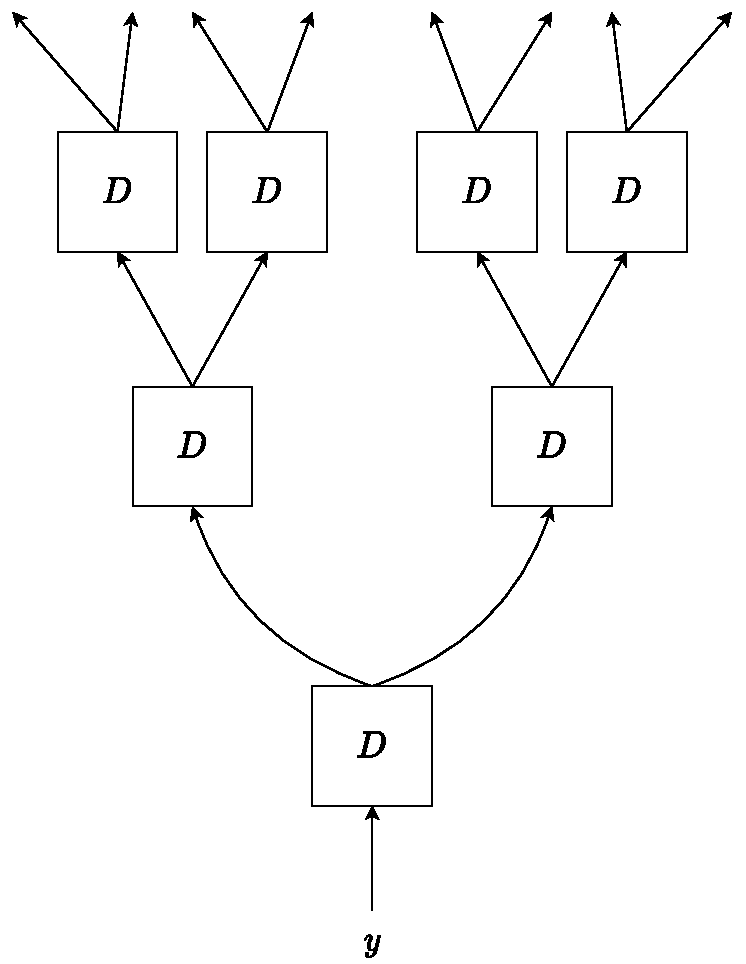
\includegraphics[width=0.4\textwidth]{j-tree.pdf}
    \captionsetup{width=1\textwidth}
    \caption{A J-tree of depth 3. Each arrow consists of $n$ wires, where $n$ is the code length of the decompressor $D$.}
    \label{fig:j-tree}
\end{figure}

We will think of a J-tree $D^k[y]$ operationally as a data structure which stores an array of $2^k$ $n$-bit values, one for each for each of its $2^k$ ``leaves'', where the $i^{th}$ value is simply $D^k[y](i)$. The state of the data structure is described purely by $y$ and $D$, which in our use cases will require far fewer bits then storing $2^k$ $n$-bit strings explicitly. In the following, we now prove that the J-tree data structure admits fast query and update operations, i.e. operations that allow us to read one entry of the data structure, or update the value of one entry. While the query operation will be computable efficiently by evaluating only the decompressor $D$ $O(k)$ times, the update operation will require evaluating some compressor $C$, and might ``fail'' in a certain well-defined sense. However, when the update does not fail, there is a deterministic algorithm which can verify, using $O(k)$ evaluations of $D$, that the resulting J-tree is in fact the true updated version of the original. We begin with the query or ``access'' operation: 
\begin{lemma}[J-tree Access Lemma]\label{lem:access}
Let $D^k[y]$ be a J-tree. Then for any $i \in \B^k$ we can compute $D^k[y](i)$ in time $O(n k)$ given $i,y$ and using $O(k)$ evaluations of $D$.
\end{lemma}
\begin{proof}
This follows directly from the definition of $D^k[y]$. Letting $b_1, \ldots, b_k$ be the individual bits of $i$, we have that:
\[
D^k[y](i) = D_{b_k} \circ D_{b_{k-1}} \circ \cdots \circ D_{b_1} (y)
\]
So we can compute $D^k[y](i)$ by evaluating $D$ $k$ times successively starting with the input $y$.
\end{proof}

\begin{definition}[J-tree Modifications]
Let $D^k[y]$, $D^k[y']$ be J-trees of depth $k$ and code length $n$. We say that the relation $\mathsf{Modified}(y,y',i,s,D)$ holds if:
\begin{enumerate}
    \item $D^k[y'](i)=s$
    \item For all $i' \in \B^k$, $i'\neq i$, $D^k[y'](i') = D^k[y](i')$
\end{enumerate}
\end{definition}
In other words, $\mathsf{Modified}(y,y',i,s,D)$ asserts that the J-tree $D^k[y']$ represents a local modification of the J-tree $D^k[y]$ which changes its $i^{th}$ value to $s$ and leaves all other values the same.
\begin{lemma}[J-tree Update Lemma]\label{lem:updates}
 There exist algorithms $\mathsf{Find}$ and $\mathsf{Verify}$ satisfying the following. 

$\mathsf{Verify}$ takes as input a decompressor $D$ (specified as an oracle) of code length $n$ and stretch 2, a pair of seeds $y,y' \in \B^n$, an index $i \in \B^k$, and a value $s \in \B^n$, and either accepts or rejects. $\mathsf{Verify}$ runs in deterministic time $O(nk)$ using $O(k)$ evaluations of $D$, and satisfies the property that if $\mathsf{Verify}(y,y',i,s,D)$ accepts, then $\mathsf{Modified}(y,y',i,s,D)$ must hold.

$\mathsf{Find}$ takes as input a compression scheme $C,D$ of code length $n$ and stretch 2 (again specified as oracles), a seed $y \in \B^n$, an index $i \in \B^k$, and a value $s \in \B^n$. It either ``succeedes'' and outputs a string $y'\in \B^n$, or else outputs $\mathsf{FAIL}\langle e \rangle$, where $e \in \B^{2n}$. $\mathsf{Find}$ runs in $O(nk)$ time using $O(k)$ evaluations of $C$ and $D$, and satisfies the property that for every input $y,i,s,C,D$, one of the following holds:
\begin{enumerate}
    \item $\mathsf{Find}(y,i,s,C,D)$ outputs a string $y'$ such that $\mathsf{Verify}(y,y',i,s,D)$ accepts.
    \item $\mathsf{Find}(y,i,s,C,D)$ outputs $\mathsf{FAIL}\langle e \rangle$, where $e$ is incompressible with respect to $C,D$.
\end{enumerate}

\end{lemma}

\begin{proof}
We start by defining the procedure $\mathsf{Find}$. Given inputs $y,i,s,C,D$, $\mathsf{Find}$ begins by computing a sequence of $k$ values $z_1, \ldots, z_k \in \B^n$ as follows. Let $b_1,\ldots,b_k$ denote the bits of $i$ in order. For each $j \in [k]$, we set
\[
z_j = D[y](b_1 b_2 \ldots b_{j-1} \lnot b_j)
\]
It is clear that the list of $z_j$ be computed in $O(nk)$ time using $O(k)$ evaluations of $D$, by storing the intermediate values of $D[y](b_1 \cdots b_j)$ for each $j$ and computing the $z_j$ in increasing order of $j$.

Now, given this list of values, we compute a second sequence $v_1,\ldots,v_k \in \B^n$. We compute the $v_j$ for each $j \in [k]$ in decreasing order of $k$ as follows. First we set:
\[
v_k = 
\begin{cases}
C(sz_k) & \text{if } b_k = 0\\
C(z_ks) & \text{if } b_k = 1
\end{cases}
\]

We then check that $D(C(sz_k)) = sz_k$ (resp. $D(C(z_ks)) = z_ks$). If this check fails we abort and return $\mathsf{FAIL}\langle sz_k \rangle$ (resp. $\mathsf{FAIL}\langle z_ks \rangle$). Now, for each $j \in \{k-1, k-2, \ldots, 1\}$, we set:
\[
v_j = 
\begin{cases}
C(v_{j+1}z_j) & \text{if } b_j = 0\\
C(z_jv_{j+1}) & \text{if } b_j = 1
\end{cases}
\]
Again, each time we evaluate $C$ on some input, we check that that input is indeed compressible with respect to $C,D$, and if not then we return $\mathsf{FAIL}\langle e\rangle$ where $e$ is the incompressible string we found. If we get to the end of this process without returning failure, we return the string $v_1$. This completes the description of the $\mathsf{Find}$ procedure, which overall requires at most $O(nk)$ time to compute using at most $O(k)$ evaluations of $C$ and $D$. Figures \ref{fig:write-f} and \ref{fig:write-b} illustrate this procedure for a J-tree of depth 3.


\begin{figure}
    \centering
    \begin{minipage}{0.45\textwidth}
        \centering
        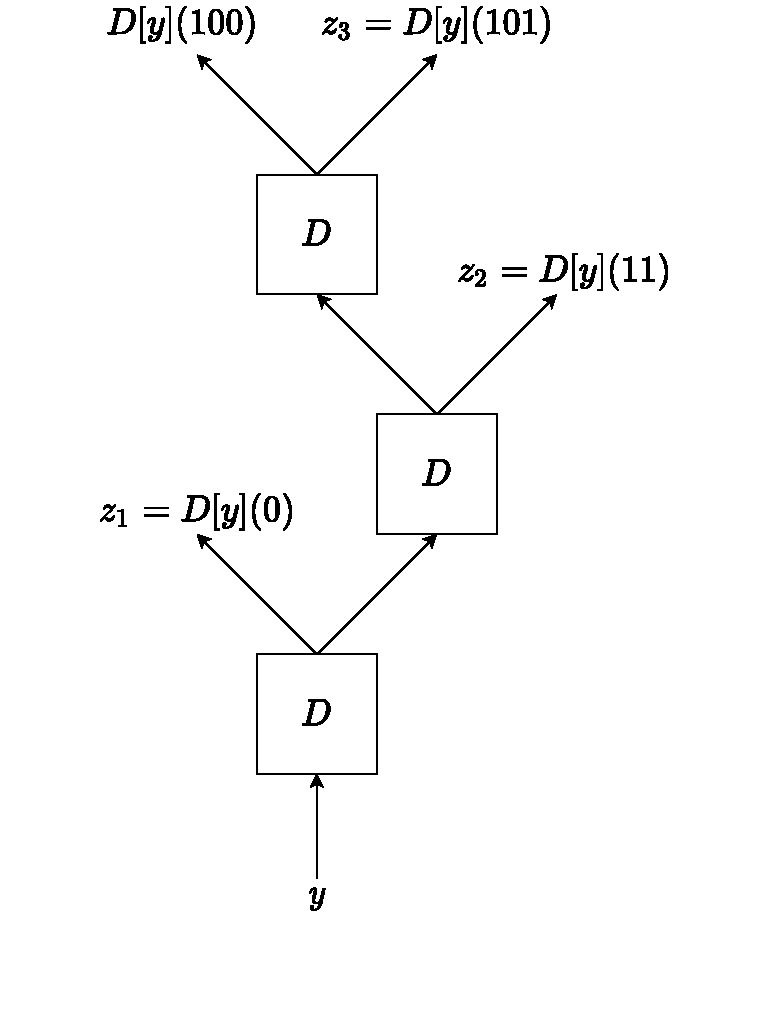
\includegraphics[width=0.8\textwidth]{write_operation_forward.pdf}
        \caption{``Forward phase'' of $\mathsf{Find}(y, 100, s,C,D)$ (where $k=3$), during which the $z_1,\ldots,z_k$ are computed.}
        \label{fig:write-f}
    \end{minipage}\hfill
    \begin{minipage}{0.45\textwidth}
        \centering
        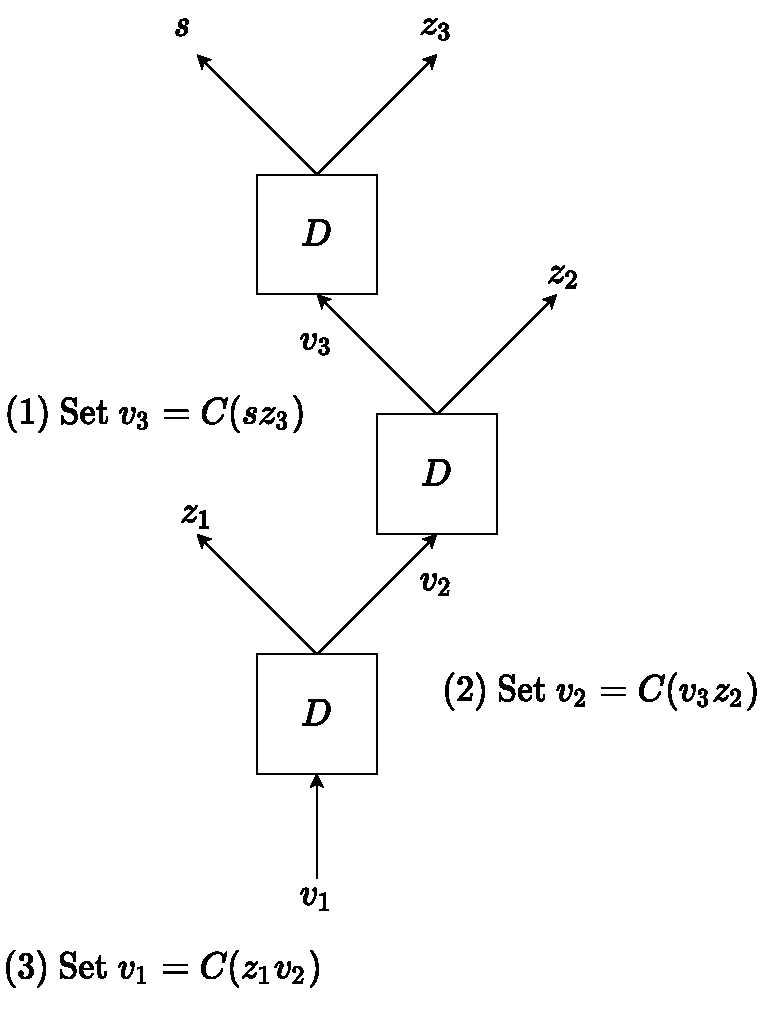
\includegraphics[width=0.8\textwidth]{write_operation_backwards.pdf} 
        \caption{``Backward phase'' of $\mathsf{Find}(y, 100, s,C,D)$ (where $k=3$), during which the $v_1,\ldots,v_k$ are computed.}
        \label{fig:write-b}
    \end{minipage}
\end{figure}


\sloppy We now describe the $\mathsf{Verify}$ procedure on input $y,y',i,s,D$, which simply verifies that a given string $y'$ is a possible successful output of $\mathsf{Find}(y,i,s,C,D)$ for some $C$. Given $y,y',i,s,D$, again let $b_1,\ldots, b_k$ denote the bits of $i$ in order. First, $\mathsf{Verify}$ iterates over each value of $j \in [k]$, and checks that $D[y'](b_1,\ldots,b_{j-1},\lnot b_j) = D[y](b_1,\ldots,b_{j-1},\lnot b_j)$. Next, it checks that $D[y'](b_1,\ldots,b_k) = D^k[y'](i) = s$. If all these conditions hold, the $\mathsf{Verify}$ procedure accepts, and otherwise it rejects. It is clear that these conditions can be verified in $O(nk)$ time using $O(k)$ evaluations of $D$, by storing the intermediate values $D[y](b_1,\ldots,b_j)$,$D[y'](b_1,\ldots,b_j)$ at each step.

We now show that if $\mathsf{Find}(y,i,s,C,D)$ succeeds and returns a string $y'$, then $\mathsf{Verify}(y,y',i,s,D)$ accepts. By definition, if $\mathsf{Find}(y,i,s,C,D)$ doesn't fail, then it is able to compute some list of values $v_1,\ldots,v_k \in \B^n$ such that for all $j < k$, $D_{b_j}(v_j) = v_{j+1}$ and $D_{\lnot b_j}(v_j) = z_j$, and it returns $v_1$ as its output. So then we have that $D[v_1](b_1,\ldots,b_{j-1},\lnot b_j) = D[v_j](\lnot b_j) = z_j$ for all $j \in [k]$. Further, we have that $D[v_1](b_1,\ldots,b_{k-1},b_k) = D[v_k](b_k) = s$. So overall $\mathsf{Verify}(y,v_1,i,s,D)$ must accept if $\mathsf{Find}(y,i,s,C,D)$ succeeds and returns $v_1$.

It remains only to show that if $\mathsf{Verify}(y,y',i,s,D)$ accepts, then $\mathsf{Modified}(y,y',i,s,D)$ must hold. Recall that $\mathsf{Modified}(y,y',i,s,D)$ asserts that the two J-trees $D^k[y]$, $D^k[y']$ agree an all indices $i'\neq i$, and that $D^k[y'](i) = s$. If $\mathsf{Verify}$ accepts then this second condition holds trivially, since $\mathsf{Verify}$ explicitly checks that $D^k[y'](i) = s$ and rejects if this does not hold. Now consider the first condition of $\mathsf{Modified}$. Let $i' \in \B^k$, $i' \neq i$. Let $\ell_1, \ldots, \ell_k$ denote the bits of $i'$ in order, and let $t \in [k]$ be the smallest index such that $\ell_t \neq b_t$. By our assumption that $\mathsf{Verify}$ accepted, we have that 
\[
D[y](\ell_1,\ldots,\ell_t) = D[y](b_1,\ldots,b_{t-1},\lnot b_t) = D[y'](b_1,\ldots,b_{t-1},\lnot b_t) = D[y'](\ell_1,\ldots,\ell_t)
\]
But by definition we also know that
\[
D[y](\ell_1,\ldots,\ell_t,\ell_{t+1},\ldots,\ell_k) = D[D[y](\ell_1,\ldots,\ell_t)](\ell_{t+1},\ldots,\ell_k)
\]
and similarly
\[
D[y'](\ell_1,\ldots,\ell_t,\ell_{t+1},\ldots,\ell_k) = D[D[y'](\ell_1,\ldots,\ell_t)](\ell_{t+1},\ldots,\ell_k)
\]
so if $D[y](\ell_1,\ldots,\ell_t) = D[y'](\ell_1,\ldots,\ell_t)$ then it must be that $D[y](\ell_1,\ldots,\ell_k) = D[y'](\ell_1,\ldots,\ell_k)$. So we have established that $D^k[y](i') = D^k[y'](i')$, which completes the proof.
\end{proof}

Next, we prove the following ``initialization'' lemma, which lets us efficiently set all leaves of a J-tree to a common value in time proportional to its depth:
\begin{lemma}\label{lem:initialization}(J-Tree Initialization Lemma)
There is an algorithm $\mathsf{Initialize}$ which takes as input a compression scheme $C,D$ of code length $n$ and stretch 2 (specified as oracles), a value $s \in \B^n$, and a depth parameter $k$. It either succeeds and returns a seed $y \in \B^n$ such that for all $i \in \B^k$, $D^k[y](i) = s$, or else outputs $\mathsf{Fail}\langle e \rangle$ where $e$ is incompressible with respect to $C,D$. $\mathsf{Initialize}(s,k,C,D)$ runs in time $O(nk)$ using $O(k)$ evaluations of $C$ an $D$.
\end{lemma}
\begin{proof}
We start by setting $v_1 = C(ss)$. When then check if $D(v_1) = ss$ and if not we return $\mathsf{Fail}\langle ss \rangle$. Otherwise we continue for each value $j \in [k]$ in increasing order, setting $v_j = C(v_{j-1}v_{j-1})$, checking that $C$ finds a valid compression at each step, and returning an incompressible string if it does not. We then return $v_k$ if all checks pass. 

Say $\mathsf{Find}(s,k,C,D)$ succeeds and returns $v_k$. By induction we show that $D[v_j](i) = s$ for all $i \in \B^j$. For the base case, since $D(v_1) = ss$ have that $D[v_1](i)=s$ for all $i \in \B$. For the inductive case say $i = bi'$ for $b \in \B, i' \in \B^{j-1}$. So then we have that $D[v_j](i) = D[D_b(v_j)](i')$. By assumption that $\mathsf{Find}(s,C,D)$ succeeds we have that $D_b(v_j) = v_{j-1}$, and by the inductive hypothesis we have that $D[v_{j-1}](i') = s$, completing the proof.
\end{proof}

In the proofs to come it will also be useful to have the following ``iterated compression'' lemma. This Lemma is implicit in the proof of the main theorem in \cite{Korten}.
\begin{lemma}[J-Tree Iterated Compression Lemma]\label{lem:compress}
 Let $C,D$ be a compression scheme of code length $n$, and let $S = (s_1, s_2, \ldots, s_{\ell})$ be a sequence of strings, where $s_i \in \B^n$. There exists an algorithm $\mathsf{Iter\dash Compress}$ running in time $poly(n,\ell)$ and using $poly(\ell)$ evaluations of $C$ and $D$ which, given $C,D$ and $S$, either ``succedes'' and outputs a seed $y \in \B^n$ such that $D^{\lceil \log \ell \rceil}[y](i) = s_i$ for all $i \in \B^{\lceil \log \ell \rceil}, i \leq \ell$, or else ``fails'' and outputs a string $e$ which is incompressible with respect to $C,D$.
\end{lemma}
\begin{proof}
This follows from repeated application of the $\mathsf{Find}$ procedure in Lemma~\ref{lem:updates}. We initialize $y=0^n$. Now, for each $i \in [\ell]$, we perform $\mathsf{Find}(y,i,s_i,C,D)$, and if $\mathsf{Find}$ fails and an incompressible string $e$, then $\mathsf{Iter\dash Compress}$ fails and outputs $e$. Otherwise we set $y = \mathsf{Find}(y,i,s_i,C,D)$. We then repeat for the next value of $i$. If we succeed for all $i$, we output the final value of $y$. Correctness and runtime of this algorithm follow from Lemma~\ref{lem:updates}.
\end{proof}

\section{Low-Space Simulations}\label{sec:low-space}
In this section we prove our main set of theorems. In each case, we show how to simulate an exponential time computation with a drastic reduction in certain resources, using short oracle calls to some uniform compression scheme. We then show that either this simulation is successful, or there is an explicit construction algorithm that prints incompressible strings for this compression scheme.


\subsection{Proofs of Main Theorems}\label{subsec:main-proofs}

\begin{theorem}\label{thm:low-space-sim}
Let $\mathcal{C},\mathcal{D} = \{C_n\}_{n \in \mathbb{N}}, \{D_n\}_{n \in \mathbb{N}}$ be a uniform compression scheme.

Then one of the following must hold:
\begin{enumerate}
    \item There is polynomial time algorithm with oracle access to $\mathcal{C},\mathcal{D}$ which, for infinitely many $n$, outputs an incompressible string for $C_n,D_n$ on input $1^n$.
    \item For every exponential time bound $T$, every language $L \in {\cl RAM\dash TIME}[T(n)]$, and every $\epsilon > 0$, there is 1-tape Turing machine with oracle access to $\mathcal{C},\mathcal{D}$ which decides $L$ in time $T(n)^{1+\epsilon}$, uses space at most $T(n)^{\epsilon}$, and makes oracle calls of length at most $T(n)^{\epsilon}$.
\end{enumerate}
\end{theorem}

\begin{proof}
Let $L \in {\cl RAM\dash TIME}[T(n)]$, and let $\mathcal{M}$ be the deterministic random access oracle machine witnessing this inclusion. Let $\mathcal{C},\mathcal{D}$ be a uniform compression scheme. By Lemma~\ref{lem:non-uniform-stretching}, we can assume $C_n,D_n$ have stretch 2 for all $n$. We will define a ``simulator machine'' which attempts to decide $L$ using low space and small oracle calls to $\mathcal{C},\mathcal{D}$. We then define a second ``checker machine'' which checks the work of the simulator. We show that whenever the simulator fails to decide $L$, the checker will be able to witness this failure in the form of an incompressible string. We will thus conclude that if simulation of $L$ fails for infinitely many inputs, the ``checker'' will constitute an explicit construction algorithm which prints incompressible strings for $\mathcal{C},\mathcal{D}$.

\subsubsection*{Step 1 - Defining the Simulator}
Let $0 < \epsilon < 1$ be a fixed rational constant. We define a machine $\mathcal{S}_{\epsilon}$ which will attempt to efficiently simulate $\mathcal{M}$ using low space, short $\mathcal{C},\mathcal{D}$-oracle queries, and which operates on a 1-tape oracle Turing machine. Let $x \in \B^n$ be an input. For the remainder of this section we will keep a particular input length $n$ fixed in our mind and thus drop the dependence of other terms on $n$ in our notation; in particular we will use the abbreviation $T = T(n)$. Our machine will now fix a particular instance of $\mathcal{C},\mathcal{D}$, in particular $C_{\lceil 2^{\epsilon n}\rceil }, D_{\lceil 2^{\epsilon n} \rceil}$; again we simplify our notation from here on and simply write $C,D$ for this scheme. By definition of a uniform compression scheme, we see that the code length of $C,D$ will by $poly(2^{\epsilon n}) = T(n)^{O(\epsilon)}$, and by assumption its message length is twice its code length. We will use $W$ to denote its code length for the remainder of the proof. 

We start by invoking Lemma~\ref{lem:ram-bst}, which lets us assume without loss of generality that $\mathcal{M}$ uses its first $T$ cells of RAM and uses at most $O(\log T)$ space on its linear tapes. This simplification will come at a $\log T$ multiplicative cost to run time, which is negligible here. Now, our simulating machine will initialize a variable $\mathtt{Mem} \in \B^W$ which will be used as a seed in a J-tree with decompressor $D$ and depth $\lceil \log T \rceil$. From now on we will fix $k = \lceil \log T \rceil$. The simulation $\mathcal{S}_{\epsilon}$ will run in $T$ phases, and will maintain the invariant that if $\mathcal{M}$'s $i^{th}$ memory cell has value $b \in \B$ at the start of $\mathcal{M}$'s $t^{th}$ time step, then $D^k[\mathtt{Mem}](i) = b^W$ at the start of $\mathcal{S}_{\epsilon}$'s $t^{th}$ phase. Aside from $\mathtt{Mem}$, $\mathcal{S}_{\epsilon}$ will also explicitly store a copy of $\mathcal{M}$'s linear tapes (which have total length $O(k)$), the input $x$, and descriptions of $\mathcal{M}$'s state and tape-head pointers, each requiring at most $k$ bits. Thus the total space required to store all local variables between phases in the simulation is at most $O(W(n)^2 + n) = T(n)^{O(\epsilon)}$ (recall that $T$ is an exponential time bound).

At the start of the first phase, $\mathcal{S}_{\epsilon}$ initializes $\mathtt{Mem}$ to a value such that $D^k[\mathtt{Mem}](i)=0^W$ for all $i \in \B^k$, which matches the initial state of $\mathcal{M}$'s RAM memory at the beginning of its computation. By Lemma~\ref{lem:initialization}, this can be accomplished in time $O(kW) = T^{O(\epsilon)}$ with oracle access to $C,D$; if the initialization procedure fails and returns an incompressible string for $C,D$, the simulation halts and rejects its input $x$. Now, in phase $t \in [T]$, $\mathcal{S}_{\epsilon}$ will simulate the $t^{th}$ step of $\mathcal{M}$ as follows:
\begin{enumerate}
    \item Read the values at the current tapehead positions on all linear tapes, and the current state of $\mathcal{M}$.
    \item Based on these values, determine which of $\mathcal{M}$'s transition rules to apply. Every rule involves a state update, which we can perform manually as we explicitly store $\mathcal{M}$'s state. If the new state is an accept/reject state for $\mathcal{M}$, then $\mathcal{S}_{\epsilon}$ halts and accepts/rejects accordingly. Otherwise:
    \begin{enumerate}
        \item First, say the rule only involves updates to the linear tapes. In this case we just carry out the rule explicitly, which requires at most $poly(k) = T^{o(\epsilon)}$ operations since the linear tapes have length $O(k)$.
        \item Next, say the rule involves a RAM operation. In this case we start by reading the entire contents of the addressing tape, which we denote $i \in \B^k$. Now, if the operation is a $\mathsf{Load}$, we compute the first bit of $D^k[\mathtt{Mem}](i)$ and update the auxiliary tape at its current tapehead position to this value. If the operation is an $\mathsf{Update}$, we read the value at the current position of the auxiliary tape, call it $s \in \B$. We then compute $\mathsf{Find}(\mathtt{Mem},i,s^W,C,D)$. If this procedure fails and returns an incompressible string, $\mathcal{S}_{\epsilon}$ aborts its entire simulation and rejects its input. Otherwise, we update $\mathtt{Mem}$ to the value returned by this $\mathsf{Find}$ call.
    \end{enumerate}
\end{enumerate}
If we get through all $T$ phases without halting, we reject the input.
\begin{figure}
    \centering
    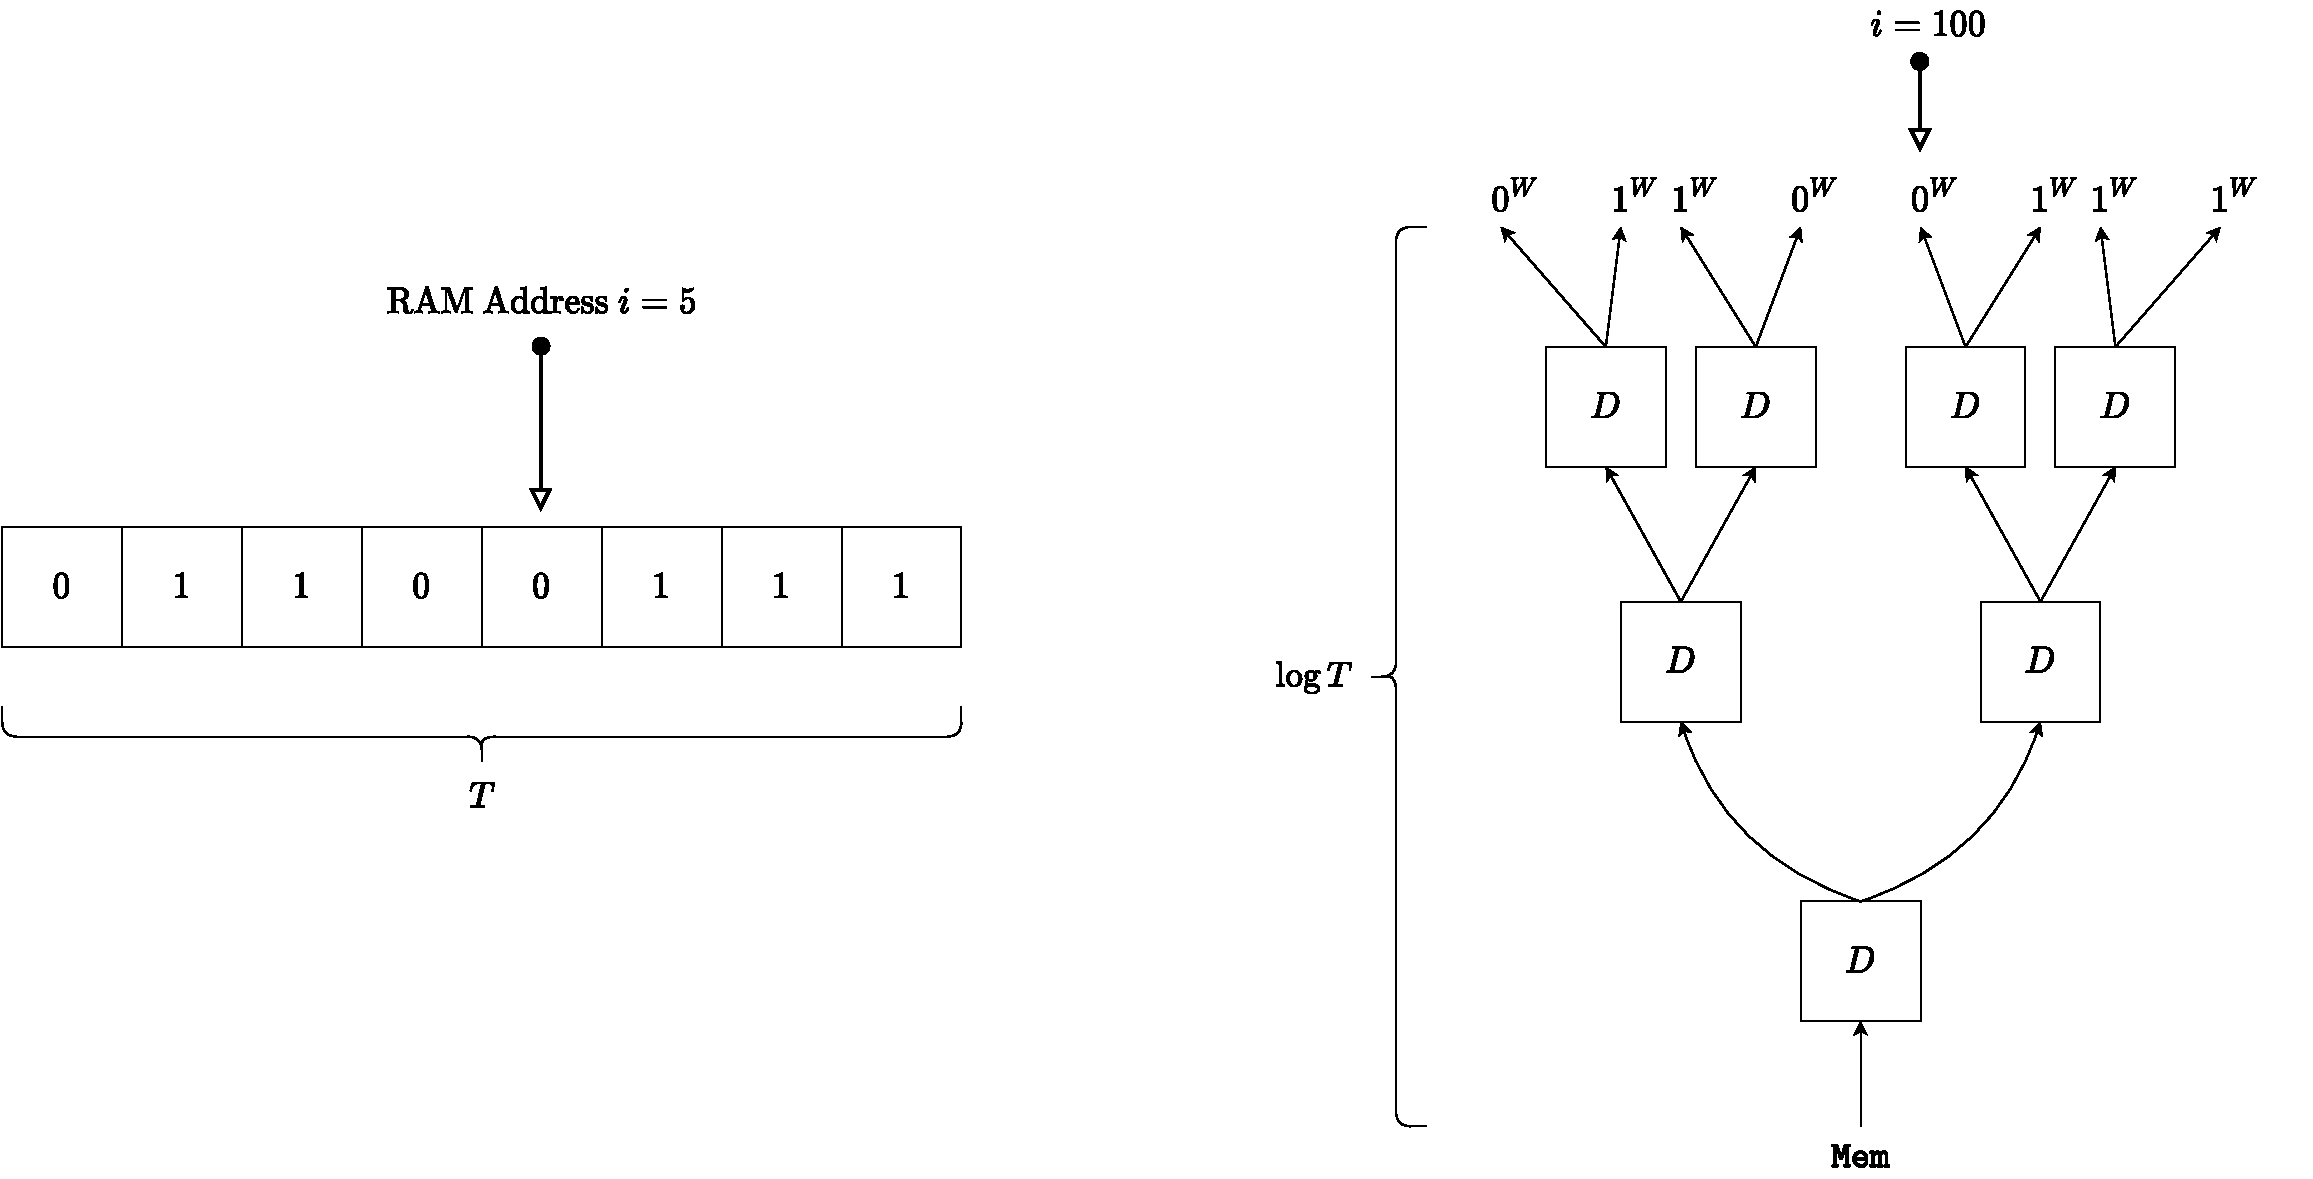
\includegraphics[width=1\textwidth]{simulation.pdf}
    \captionsetup{width=1\textwidth}
    \caption{Simulating a RAM memory with a J-tree. While the RAM memory on the left requires $T$ bits to store explicitly, the virtual RAM on the right can be stored with $|\mathtt{Mem}| = W = T^{O(\epsilon)}$ bits.}
    \label{fig:simulation}
\end{figure}

We now show that $\mathcal{S}_{\epsilon}$ operates within the required resource bounds. First, we note that all oracle calls are of length $W = T^{O(\epsilon)}$. Second, it is clear that the $\mathsf{Find}$/$\mathsf{Initialize}$ operations and the evaluations of $D^k[\mathtt{Mem}]$ can be carried out in $poly(W)$ space, since in particular they require at most $poly(W)$ time by Lemmas~\ref{lem:access}, \ref{lem:updates}, and \ref{lem:initialization}. So the space used within a phase is at most $poly(W) = T^{O(\epsilon)}$ and the size of oracle calls are bounded identically. To bound the time complexity, we note that by the same arguments each phase can be completed in time $T^{O(\epsilon)}$, and overall there are $T$ phases, so the total time complexity is $T^{1 + O(\epsilon)}$. In the above description of each phase, we were informal about the number of work tapes required to carry out these computations. However, since any multi-tape machine running in space $S$ and time $T$ can be simulated on a one-tape machine in time $poly(S,T)$ and space $poly(S)$, we see that we can modify the algorithm within each phase to operate on a 1-tape machine with at most a polynomial blowup in space and time. So the above bounds still hold on a 1-tape machine, where the space is bounded by $poly(T^{\epsilon})= T^{O(\epsilon)}$, and the time within each phase is bounded identically.

\subsubsection*{Step 2 - If $\mathsf{Find}$ Never Fails Then the Simulator Works}
We now show that if $\mathcal{S}_{\epsilon}$ completes its computation on an input $x$ without any $\mathsf{Initialize}$ or $\mathsf{Find}$ operation failing, then $\mathcal{S}_{\epsilon}$ accepts $x$ if and only if $x \in L$. To prove this, we show by induction on $t \in [T]$ that at the beginning of the $t^{th}$ phase of $\mathcal{S}_{\epsilon}$'s simulation on $x$, $\mathcal{S}_{\epsilon}$'s simulated configuration matches the configuration of $\mathcal{M}$ on input $x$ at the beginning of time step $t$. This is clearly true for $t = 1$, since at the start of the simulation we initialize explicit representations of $\mathcal{M}$'s linear tapes to all zeroes, and do the same for the RAM memory using the $\mathsf{Initialize}$ operation, which succeeds by assumption.

Now assume the inductive hypothesis up to step $t$. So at the beginning of this time step on input $x$, $\mathcal{M}$'s linear tapes, tapehead pointers, machine state and RAM memory at the start of time step $t$ are faithfully represented by $\mathcal{S}_{\epsilon}$ at the start of phase $t$. Thus, $\mathcal{S}_{\epsilon}$ is able to choose the correct transition rule to apply during this phase. It then updates the linear tapes, tapehead pointers, and machine state accordingly; all of these are stored explicitly so $\mathcal{S}_{\epsilon}$ has no potential for failure here. Next, if $\mathcal{M}$ uses a $\mathsf{Load}$ operation at this step, since we assumed the previous state of the virtual RAM is accurate, the correct value will be found by $\mathcal{S}_{\epsilon}$. Finally, if $\mathcal{M}$ uses a $\mathsf{Update}$ operation at this step, $\mathcal{S}_{\epsilon}$ makes the associated call to the $\mathsf{Find}$ procedure. By Lemma~\ref{lem:updates}, if this does not fail, then the state of the virtual RAM after this step will accurately represent $\mathcal{M}$'s ram at the end of time step $t$. This completes the inductive case.

\subsubsection*{Step 3 - Failure of the Simulator Witnesses the Pigeonhole Principle for $\mathcal{C},\mathcal{D}$}

We now show that if the above simulation $\mathcal{S}_{\epsilon}$ fails to decide $L$ for infinitely many inputs, then there is an algorithm which, given $1^n$, outputs an incompressible string for $C_n,D_n$ in polynomial time using oracles for $\mathcal{C},\mathcal{D}$, for infinitely many $n$.

In particular, assume that there is an infinite set $R \subseteq \mathbb{N}$ such that for all $n \in R$, $\mathcal{S}$ makes a mistake on some length $n$ input in its attempt to decide $L$. Recall that $\mathcal{S}_{\epsilon}$ uses the compression scheme $C_{\lceil 2^{\epsilon n} \rceil}, D_{\lceil 2^{\epsilon n} \rceil}$ in its simulation on inputs of length $n$. Now, let $\mathbb{I} = \{\lceil 2^{\epsilon n} \rceil \mid n \in R\}$. We will give a construction algorithm that succeeds for all input lengths in $\mathbb{I}$. 

Given an input $1^m$, our construction algorithm $\mathcal{H}$ operates as follows. It starts by computing an $n$ such that $\lceil 2^{\epsilon n} \rceil = m$; by construction we see $n = O(\log m)$. Next, $\mathcal{H}$ runs the simulation $\mathcal{S}_{\epsilon}$ on all inputs of length $n$ one after the other; by construction we see that $\mathcal{S}_{\epsilon}$ uses the same compression scheme $C_m,D_m$ on all such inputs. During each simulation, if $\mathcal{S}_{\epsilon}$ fails on some $\mathsf{Find}$ or $\mathsf{Initialize}$ operation and returns an incompressible string for $C_m,D_m$, $\mathcal{H}$ halts and outputs that string. If $\mathcal{H}$ gets through all inputs of length $n$ without any operation failing, it outputs something arbitrary, say $1^m$. By definition we see that when $m \in \mathbb{I}$, $\mathcal{H}$ cannot get through all simulations without $\mathcal{S}_{\epsilon}$ failing, since by definition of $\mathbb{I}$ we know that $\mathcal{S}_{\epsilon}$ fails to compute $L$ on some input of length $n$, and by the previous section we know this can only happen when $\mathcal{S}_{\epsilon}$ fails on some $\mathsf{Find}$/$\mathsf{Initialize}$ operation. So overall we have that $\mathcal{H}$ runs in $poly(2^n) = 2^{O(n)} = 2^{O(\log m)} = poly(m)$ time, and successfully finds an incompressible string for $C_m,D_m$ on input $1^m$ for infinitely many $m$.

\subsubsection*{Step 4 - Wrapping Things Up}
We now have that for any language $L \in {\cl RAM\dash TIME}[T(n)]$ and every $\epsilon > 0$, there is a machine $S_{\epsilon}$ running in time $T(n)^{1+O(\epsilon)}$, space $T^{O(\epsilon)}$, and making $\mathcal{C},\mathcal{D}$ oracle calls of length $T^{O(\epsilon)}$, such that one of the following holds:
\begin{enumerate}
    \item $\mathcal{S}_{\epsilon}$ correctly decides $L$ on all but finitely many inputs.
    \item There is a polynomial time construction algorithm which finds incompressible strings for $C_n,D_n$ given oracles for $\mathcal{C},\mathcal{D}$, which works for infinitely many inputs.
\end{enumerate}
Clearly if the first possibility  holds then we can get a simulation of the same complexity which decides $L$ exactly. In addition, if the first possibility holds for all $\epsilon > 0$, then we can replace the $O(\epsilon)$ terms with $\epsilon$ as we take $\epsilon$ to zero. This yields the stated theorem.
\end{proof}

We now prove a variant of the above theorem, which allows us to replace the oracle for the compressor $\mathcal{C}$ in our low-space simulation with nondeterminism. This will be relevant for schemes $\mathcal{C},\mathcal{D}$ where $\mathcal{C}$ is significantly harder to compute then $\mathcal{D}$.
\begin{theorem}\label{thm:swap-d-for-np}
Let $T$ be an exponential time bound, and let $\mathcal{C},\mathcal{D}$ be a uniform compression scheme.

Then one of the following must hold:
\begin{enumerate}
    \item There is polynomial time algorithm with oracle access to $\mathcal{C},\mathcal{D}$ which, for infinitely many $n$, outputs an incompressible string for $C_n,D_n$ on input $1^n$.
    \item For every language $L \in {\cl RAM\dash TIME}[T(n)]$ and every $\epsilon > 0$, there is nondeterministic 1-tape Turing machine with oracle access to $\mathcal{D}$ which decides $L$ in time $T(n)^{1+\epsilon}$, uses space at most $T(n)^{\epsilon}$, and makes at most $T(n)^{\epsilon}$ nondeterministic guesses on all computation paths.
\end{enumerate}
\end{theorem}
\begin{proof}
We follow the same simulation $\mathcal{S}_{\epsilon}$ of some language $L$ in ${\cl RAM\dash TIME}[T(n)]$, with a slight modification. The key observation is the following: the procedure $\mathsf{Find}$ is proven to work with access to both $\mathcal{C}$ and $\mathcal{D}$ oracles by Lemma~\ref{lem:updates}. However, recall that Lemma~\ref{lem:updates} also defines separate procedure $\mathsf{Verify}$, which is able to verify that a certain J-tree seed is the updated form of another, and this verification only needs the $\mathcal{D}$ oracle. Recall also the key property relating $\mathsf{Find}$ and $\mathsf{Verify}$, which says that $\mathsf{Verify}$ will accept any successful output of a $\mathsf{Find}$ operation.

Thus, if we make our simulator $\mathcal{S}_{\epsilon}$ nondeterministic, it can replace the $\mathsf{Find}$ operation by a nondeterministic guess as to the new value of the seed $\mathtt{Mem}$ during each phase, and then use $\mathsf{Verify}$ to check that this guess is correct, which requires only the $\mathcal{D}$ oracle. This immediately gives us a low space nondeterministic simulator $\mathcal{S}_{\epsilon}$ with similar properties as that in the proof of Theorem~\ref{thm:low-space-sim}. However, the total nondeterminism used by this simulation is $T(n)^{1 + O(\epsilon)}$, since it has to guess a seed of length $T^{O(\epsilon)}$ during each of the $T$ phases. 

To get away with $T^{O(\epsilon)}$ bits of nondeterminism, we use the following trick\footnote{This trick is essentially the ``easy witness method'' of \cite{Kabenets}.}. At the beginning of $\mathcal{S}_{\epsilon}$'s simulation, it guesses a single seed for a separate J-tree of the same code length, call this seed $\mathtt{Up}$. Now, during phase $t$, to simulate an $\mathsf{Update}$ operation which sets RAM cell $i \in \B^k$ to value $s \in \B$, we first set $\mathtt{Mem}' = D^k[\mathtt{Up}](t)$, and then check if $\mathsf{Verify}(\mathtt{Mem}, \mathtt{Mem}', i, s^W, D)$ holds. If so we then set $\mathtt{Mem} = \mathtt{Mem}'$ and continue to the next phase, and if not then we halt the simulation and reject outright. It is straightforward to see that this simulation runs in time $T(n)^{1 + O(\epsilon)}$, uses space $T(n)^{O(\epsilon)}$, and guesses at most $T(n)^{O(\epsilon)}$ nondeterministic bits.

By the same arguments as in Theorem~\ref{thm:low-space-sim}, we have that if every $\mathsf{Verify}$ call accepts during $\mathcal{S}_{\epsilon}$'s computation on input $x$, then $\mathcal{S}_{\epsilon}$ correctly decides if $x \in L$. To finish the proof, it suffices to show that given some $x$ such that $\mathcal{S}_{\epsilon}$ fails to decide if $x \in L$, we can construct an incompressible string for $C_{2^{\epsilon n}}, D_{2^{\epsilon n}}$ in $poly(T(n))$ time with $\mathcal{C}, \mathcal{D}$ oracles; from here the theorem follows directly using the arguments at the end of the proof of Theorem~\ref{thm:low-space-sim}. 

So, say we have such an $x$. Since our simulation errs on the side of rejecting, we know that $x \in L$ but $\mathcal{S}_{\epsilon}$ rejects $x$. We start by running the \emph{deterministic} low space simulation from Theorem~\ref{thm:low-space-sim} (corresponding to $L, \epsilon$) on $x$, which can be done in $poly(T(n))$ time with $\mathcal{C},\mathcal{D}$ oracles. During this simulation, we keep track of all updated memory seeds constructed using $\mathsf{Initialize}$ and $\mathsf{Find}$. If at any step a $\mathsf{Find}$ or $\mathsf{Initialize}$ procedure fails, we find an incompressible string and output it. Otherwise, we have found a sequence of seeds $\mathtt{Mem}_1, \ldots, \mathtt{Mem}_T \in \B^W$ (where $W$ is the code length used by the simulation), such that $\mathtt{Mem}_{t+1}$ represents a correct update to the RAM memory previously represented by $\mathtt{Mem}_t$ after time step $t$. Now, we use the $\mathsf{Iter\dash Compress}$ procedure to construct a seed $\mathtt{Up} \in \B^W$ such that for all $t \in \B^k$, $D^k[\mathtt{Up}](t) = \mathtt{Mem}_t$. By Lemma~\ref{lem:compress}, in $poly(T(n))$ time we can either find such a seed $\mathtt{Up}$, or else find an incompressible string for our scheme. But if such a string $\mathtt{Up}$ exists, this is precisely the nondeterministic guess which would cause our nondeterministic simulation $\mathcal{S}_{\epsilon}$ to accept $x$. So by assumption that it rejects $x$, if we get to this point then $\mathsf{Iter\dash Compress}$ must find an incompressible string.
\end{proof}
Finally, we show that if the explicit construction algorithm in the above theorem is also granted access to an {\cl NP} oracle, we can get the same result, but where we simulate languages in the larger class ${\cl NTIME}[T(n)]$.
\begin{theorem}\label{thm:full-ntisp-sim}
Let $T$ be an exponential time bound, and let $\mathcal{C},\mathcal{D}$ be a uniform compression scheme.

Then one of the following must hold:
\begin{enumerate}
    \item There is polynomial time algorithm with oracle access to $\mathcal{C},\mathcal{D}$, and ${\sc SAT}$ which, for infinitely many $n$, outputs an incompressible string for $C_n,D_n$ on input $1^n$.
    \item For every language $L \in {\cl NTIME}[T(n)]$ and every $\epsilon > 0$, there is nondeterministic 1-tape Turing machine with oracle access to $\mathcal{D}$ which decides $L$ in time $T(n)^{1+\epsilon}$, uses space at most $T(n)^{\epsilon}$, and makes at most $T(n)^{\epsilon}$ nondeterministic guesses on all computation paths.
\end{enumerate}
\end{theorem}
\begin{proof}
This will follow quite directly from the proof of the previous theorem. Let $\mathcal{M}$ be some ${\cl NTIME}[T(n)]$ machine which we are attempting to simulate. At the outset of its computation, in addition to guessing one seed $\mathtt{Up}$ which encodes a sequence of RAM-seed updates, our new simulator $\mathcal{S}_{\epsilon}$ also guesses a second seed $\mathtt{Wit}$ which will encode the nondeterministic choices made by $\mathcal{M}$ during its computation. In particular, after guessing this seed, at each phase $t$ of our simulation the simulator reads the first $O(1)$ bits of $D^k[\mathtt{Wit}](t)$, and uses this to determine which transition rule to apply at that step (in a nondeterministic machine there can be $O(1)$ such rules, which will be smaller then the code length of the decompressor for sufficiently large input lengths). Otherwise we run the simulation exactly as in the above proof.

By the same reasoning as in the previous proof, we see that if this machine accepts an input $x$ then $x \in L$ (since the simulation errs on the side of rejection), but it is possible that $x \in L$ and the simulation fails to determine this. In such a case, the only possibility is that for all sequences $z \in \B^{O(T)}$ of nondeterministic guesses causing $\mathcal{M}$ to accept $x$, there is no pair $\mathtt{Up},\mathtt{Wit} \in \B^W$ such that $\mathtt{Wit}$ encodes $z$ (as described above), and $\mathtt{Up}$ encodes a sequence of valid RAM seeds representing the deterministic computation of $\mathcal{M}$ on $x$ with witness $z$. Thus, if we have some input $x$ on which our simulation fails, we can use an {\cl NP} oracle to compute a witness $z$ causing $\mathcal{M}$ to accept $x$. We then run the deterministic low space simulation $\mathcal{M}$ on $x$ with witness $z$, and either find an incompressible string for $\mathcal{C},\mathcal{D}$, or else find a sequence of valid RAM seeds $\mathtt{Mem}_1,\ldots,\mathtt{Mem}_T$ for this computation. We then proceed as in the previous Theorem, attempting to compress the $\mathtt{Mem}_t$ to a single seed $\mathtt{Up}$ and the bits of $z$ to another seed $\mathtt{Wit}$, both using the $\mathsf{Iter\dash Compress}$ procedure. By assumption that our main nondeterministic simulation rejected $x$, if we get to this point we know that one of these $\mathsf{Iter\dash Compress}$ procedures must return an incompressible string. 
\end{proof}


\subsection{Implications}\label{subsec:implications}

Consider the following three hypotheses:
\begin{hypothesis}\label{hyp:tisp-lb}
There exists some exponential time bound $T$ and some $\epsilon > 0$ such that:
\[
{\cl RAM\dash TIME}[T(n)] \not\subseteq {\cl 1\dash TISP}[T(n)^{1+\epsilon}, T(n)^{\epsilon}]
\]
\end{hypothesis}
\begin{hypothesis}\label{hyp:ntisp-lb}
There exists some exponential time bound $T$ and some $\epsilon > 0$ such that:
\[
{\cl NTIME}[T(n)] \not\subseteq {\cl 1\dash NTISPG}[T(n)^{1+\epsilon}, T(n)^{\epsilon}, T(n)^{\epsilon}]
\]
\end{hypothesis}

\begin{hypothesis}\label{hyp:strong-ntisp-lb}
There exists some exponential time bound $T$ and some $\epsilon > 0$ such that:
\[
{\cl RAM\dash TIME}[T(n)] \not\subseteq {\cl 1\dash NTISPG}[T(n)^{1+\epsilon}, T(n)^{\epsilon}, T(n)^{\epsilon}]
\]
\end{hypothesis}

The first Hypothesis asserts that deterministic exponential time RAM computations cannot be simulated on 1-tape machines using low space and near-linear blowup in time. The second Hypothesis asserts roughly the same for nondeterministic computations, claiming that such a simulation cannot occur which simultaneously uses a small amount of nondeterminism. Recall that for nondeterministic time, the multi-tape and RAM models are roughly equivalent, which is why we don't make a distinction here on the left-hand side. Finally, the third hypothesis says that deterministic RAM computations cannot be recognized by machines with short ``proofs'' verifiable in low space and near-linear time on a 1-tape machine.

While \ref{hyp:tisp-lb} and \ref{hyp:ntisp-lb} seem incomparable and both quite reasonable, we see that \ref{hyp:strong-ntisp-lb} is formally stronger then the previous two, and we have significantly less intuition as to whether or not it should be true. However, recall from Section~\ref{subsec:known-tradeoffs} that when the time bound $T$ is linear, all three of these hypotheses are known to hold unconditionally (indeed they hold for \emph{all} $\epsilon < 1$). In any case, the results of the previous section give us the following:
\begin{theorem}\label{thm:tisp-impl}
If Hypothesis~\ref{hyp:tisp-lb} holds, then for any uniform compression scheme $\mathcal{C},\mathcal{D}$ where both $\mathcal{C}$ and $\mathcal{D}$ are computable in polynomial time, there is a polynomial time algorithm which, given $1^n$, prints an incompressible string for $C_n,D_n$ for infinitely many $n$.
\end{theorem}
\begin{proof}
This follows from Theorem~\ref{thm:low-space-sim}; since the $\mathcal{C}$ and $\mathcal{D}$ oracle calls are of length $T(n)^{O(\epsilon)}$, if both $\mathcal{C}$ and $\mathcal{D}$ are computable in polynomial time then the oracles can be abandoned without effecting the resource bounds of the simulation.
\end{proof}
For Hypothesis 2, we have:
\begin{theorem}\label{thm:full-ntisp-impl}
If Hypothesis~\ref{hyp:ntisp-lb} holds, then for any uniform decompressor $\mathcal{D}$ computable in polynomial time, there exists there is a polynomial time {\cl NP}-oracle algorithm which, given $1^n$, prints an empty pigeonhole for $D_n$ for infinitely many $n$. In particular, ${\cl E}^{\cl NP} \not\subseteq {\cl size}[2^n/2n]$.
\end{theorem}
\begin{proof}
This follows from Theorem~\ref{thm:full-ntisp-sim}. As noted in Section~\ref{sec:pigeons}, any polynomial time decompressor $\mathcal{D}$ has a canonical ``proper compressor'' $\mathcal{C}$ computable with an {\cl NP} oracle, such that the incompressible strings for this scheme are empty pigeonholes for $\mathcal{D}$. The theorem then follows from the above proof, where we can abandon the $\mathcal{D}$ oracle in our simulation if $\mathcal{D}$ is computable in polynomial time since the oracle calls we make are small.
\end{proof}

Finally, the strongest hypothesis gives us the following:
\begin{theorem}\label{thm:swap-d-impl}
If Hypothesis~\ref{hyp:strong-ntisp-lb} holds, then for any uniform compression scheme $\mathcal{C},\mathcal{D}$ where $\mathcal{D}$ is computable in polynomial time, there is a polynomial time algorithm using a $\mathcal{C}$ oracle which, given $1^n$, prints an incompressible string for $C_n,D_n$ for infinitely many $n$.
\end{theorem}
\begin{proof}
This follows from Theorem~\ref{thm:swap-d-for-np}, where again we use the fact that $\mathcal{D}$ is computable in polynomial time to eliminate the $\mathcal{D}$ oracle.
\end{proof}

To illustrate the use of these theorems, we first consider their implications for the compression schemes related to non-uniform complexity measures described in Section~\ref{subsubsec:tt-gens}. In these cases, we have some complexity measure on strings/truth tables, such as circuit complexity, formula size, or $K^{poly}$ complexity, and wish to construct strings/truth tables of high complexity (for infinitely many input lengths), which we call the ``construction problem.'' In each case there is an associated ``compression problem'' in {\cl FNP}, where we are given a string/truth table and wish to find a small circuit/formula/program computing it if one exists. For these sorts of problems, we now have the following:
\begin{corollary}\label{cor:main-impls}
For each of the above mentioned uniform compression schemes related to non-uniform complexity measures, we have:
\begin{enumerate}
    \item If Hypothesis~\ref{hyp:tisp-lb} holds, then an efficient algorithm for the compression problem implies an efficient algorithm for the construction problem.
    \item If Hypothesis~\ref{hyp:ntisp-lb} holds, then there is an efficient {\cl NP}-oracle algorithm for the construction problem.
    \item If Hypothesis~\ref{hyp:strong-ntisp-lb} holds, then there is an efficient algorithm for the construction problem using an arbitrary oracle for the compression problem. In other words, the construction problem reduces to the compression problem.
\end{enumerate}
\end{corollary}
\begin{proof}
The first and second implications follow directly from the above theorems. For the last implication, there is a slight subtlety  related to the fact that the compression problem can generally have many valid solutions per instance, and so an oracle for this problem must be defined according to our notion of ``functional oracles'' (defined in Section~\ref{subsec:search-problems}). Thus, for a particular compression problem we have the following dichotomy for every one of its function oracles $\mathcal{O}$: either the compression scheme defined by $\mathcal{O}$ returns solutions that can be used as witnesses in the low space simulation for all but finitely many inputs, or else there is an explicit construction algorithm with access to $\mathcal{O}$ which prints strings of high complexity. So assuming Hypothesis~\ref{hyp:strong-ntisp-lb}, every $\mathcal{O}$ must fail to help the simulation for infinitely many inputs. Thus, given access to an arbitrary functional oracle for the compression problem, the explicit construction algorithm will work for infinitely many input lengths, although the choice of functional oracle might affect which infinite set of input lengths the algorithm works on.
\end{proof}
We see here that the conclusion of the third implication implies the conclusion of the previous two. As noted in the introduction, the second implication can be proved by simpler techniques, utilizing the ``Easy Witness Lemma.'' We give an alternate proof using this method in Appendix~\ref{appendix:ewl} for the interested reader. However, for the first and third implication, the J-tree update lemma seems necessary.

The case of large prime construction does not quite fit in with the others, as both the compressor and decompressor given in Theorem~\ref{thm:primes-in-apepp} require a factoring oracle. In addition, the second implication of Corollary~\ref{cor:main-impls} above is trivial when applied to the construction of large primes, since primality testing is in {\cl P} \cite{primes}. However we can still derive the following from Theorem~\ref{thm:tisp-impl}:
\begin{corollary}\label{cor:prime-construction}
If Hypothesis~\ref{hyp:tisp-lb} holds, then a polynomial time algorithm for factoring implies a polynomial time algorithm to construct $16n$-bit primes of magnitude $>2^n$ (for infinitely many $n$).
\end{corollary}

More generally we can conclude the following directly from Theorem~\ref{thm:low-space-sim}:
\begin{corollary}\label{cor:factoring-oracle}
One of the following is true:
\begin{enumerate}
    \item For every exponential time bound $T$ and every $\epsilon>0$, every language decidable in time $T(n)$ on a RAM machine can be decided in time $T(n)^{1+\epsilon}$ and space $T(n)^{\epsilon}$ by a 1-tape machine with a factoring oracle, which makes oracle calls of length at most $T(n)^{\epsilon}$.
    \item There is a polynomial time algorithm with a factoring oracle that generates $32n$-bit primes of magnitude $>2^n$ for infinitely many $n$.
\end{enumerate}
\end{corollary}
\section{BPP, TFNP, and the Weak Pigeonhole Principle}\label{sec:bpp}
Throughout this paper we have studied the problem of finding incompressible strings for \emph{uniform} compression schemes. As mentioned in Section~\ref{sec:pigeons}, it would also be natural to study the more general search problem, where a compression scheme of a fixed message/code length is given as input in the form of a boolean circuit:
\begin{definition}
{\sc Lossy Code} is the following problem: given circuits $C\colon \B^n \rightarrow \B^{n-1}$ and $D\colon \B^{n-1} \rightarrow \B^n$, find some $x$ such that $D(C(x)) \neq x$.
\end{definition}
It follows from the definition that {\sc Lossy Code} lies in {\cl TFNP} (more specifically the class {\cl PPP} defined in \cite{christos}), and reduces to the problem {\sc Empty} studied in \cite{total} and \cite{Korten}. Further, we have seen that {\sc Lossy Code} admits a randomized algorithm that outputs a solution with high probability. Since solutions can be verified efficiently, this fits it into a family of search problems studied by Goldreich \cite{Goldreich}, whose results imply the following:
\begin{lemma}
{\sc Lossy Code} is polynomial time Turing reducible to {\sc CAPP}.
\end{lemma}

Here, {\sc CAPP} denotes the canonical complete problem for {\cl prBPP}, where we are given as input a circuit $E\colon \B^n \to \B$, and must output an approximation of $Pr_x[E(x)=1]$ that is accurate to within $\pm \frac{1}{6}$.
A natural question is whether the converse holds, i.e. whether {\sc CAPP} reduces deterministically to {\sc Lossy Code}. As hinted towards in Section~\ref{subsec:particular-pairs}, a polynomial time algorithm for {\sc Circuit Synthesis} would imply such a reduction, but an unconditional reduction would be a major breakthrough as it would place ${\cl BPP} \subseteq {\cl NP}$. We show here that if the compressor $C$ in {\sc Lossy Code} is allowed to be randomized, the associated total search problem is in fact Turing-equivalent to {\sc CAPP}, and thus complete for {\cl prBPP}. The problem is defined formally as follows:

\begin{definition}
{\sc R-Lossy Code} is the following problem: given $C\colon \B^n \times \B^m \rightarrow \B^{n-1}$, $D\colon \B^{n-1} \rightarrow \B^n$, find some $x \in \B^n$ such that $Pr_r[D(C(x,r)) = x] < \frac{1}{2}$.
\end{definition}
To clarify, this is precisely the same problem as {\sc Lossy Code}, except that the ``compressor circuit'' $C$ now uses some random coins. In this case, we seek a string which has a $<\frac{1}{2}$ probability of being recoverable from its description (where the probability is taken over the random coins of the compressor $C$). Just like {\sc Lossy Code} this search problem is total, but verifying a solution is no longer in {\cl P}. Indeed, it may be {\cl PP}-hard to determine if any particular string is a solution, but there is a efficient randomized verification procedure that accepts only valid solutions, and accepts a random solution with high probability.

We now show the following:
\begin{theorem}\label{thm:bpp-pigeon}
{\sc R-Lossy Code} and {\sc CAPP} are Turing reducible to one another in deterministic polynomial time.
\end{theorem}
\begin{proof}
A reduction from {\sc R-Lossy Code} to {\sc CAPP} follows from \cite{Goldreich}. To see this, note that a random $x \in \B^n$ is an empty pigeonhole for $D$ with probability $\geq \frac{1}{2}$, and whenever $x$ is an empty pigeonhole we have $Pr_r[D(C(x,r))=x] = 0$. In contrast, when $x$ is a non-solution we have $Pr_r[D(C(x,r))=x] \geq \frac{1}{2}$. So distinguishing empty pigeonholes from non-solutions is a problem in {\cl prBPP} (indeed its lies in {\cl prRP}), there is an efficient randomized algorithm which generates empty pigeonholes with high probability (namely the trivial algorithm that outputs a random $x$), and any empty pigeonhole is a solution. This problem therefore falls into the category of search problems which were proven reducible to {\sc CAPP} in \cite{Goldreich}.

To get a reduction in the other direction, we rely on Yao's next-bit predictor lemma \cite{Yao}. In particular, say we are given a circuit $E \colon \B^n \to \B$ whose acceptance probability we wish to estimate to within an additive error of $\frac{1}{6}$. By Yao's lemma, for any sufficiently large table of $n$-bit strings $A \in \B^{m \times n}$ we have that if $E$'s acceptance probability over the rows of $A$ differs from its true acceptance probability over $\B^n$ by more than $\frac{1}{6}$, then there is a simple ``predictor circuit'' which uses $E$ to derive one of the columns of $A$ from its remaining columns. In particular, this argument shows that there is some small advice of length $<mn$ from which we can reconstruct $A$ (whose original bit-length is $mn$) using $E$. This immediately implies a reduction to {\sc Empty} as described in \cite{Korten}. The key observation we make here (which is also noted in several other works on the subject, notably \cite{CIKK} and \cite{Hirahara}) is that the ``compressed representation'' of $A$ described in this argument can indeed be \emph{found efficiently given $E$} using randomness. This will imply a reduction of {\sc CAPP} to {\sc R-Lossy Code}, since any table $A$ which cannot be recovered from this randomized compression procedure will then give a good approximation to $E$'s acceptance probability.

More formally, given $E$ as above we will construct an instance of {\sc R-Lossy Code} with message length $n^5$ and code length $n^5-1$. The compressor circuit $C\colon \B^{n^5} \times \B^{poly(n)} \to \B^{n^5-1}$ interprets its $n^5$-bit input as an $n^4 \times n$ matrix. $C$ then iterates over all choices $i \in [n], b \in \B$ of a ``hybrid index'' and ``bias.'' For each such choice, let $x^{<i}_1,\ldots,x^{<i}_m$ denote the rows of $A$ truncated to their first $i-1$ bits. Our compressor now selects a random $z \in \B^{n - i + 1}$, and attempts to predict the $i^{th}$ column of $A$ from the preceding columns as follows: it predicts the $j^{th}$ value of the $i^{th}$ column of $A$ to be the first bit of $z$ if $E(x^{<i}_j z)= b$, or else the negation of this first bit if $E(x^{<i}_j z)\neq b$. Given a particular selection of $i,b$ and $z$, the compressor then evaluates the accuracy of this prediction, by counting the number of correctly guessed entries of the $j^{th}$ column of $A$. If it guesses fewer than $\frac{n^4}{2} + \frac{n^3}{12}$ correctly, $C$ aborts and outputs something arbitrary. If $C$ guesses at least $\frac{n^4}{2} + \frac{n^3}{12}$ correctly, it then sets $q \in \B^{n^4}$ equal to the bit-wise XOR of the correct column and the predicted column. Since in this case $q$ will be an $n^4$-bit string with weight at most $\frac{n^4}{2}-\frac{n^3}{12}$, we can then encode $q$ in $n^4-\Omega(n^2)$ bits using a standard sparse-string encoding scheme \cite{Korten}. Finally, the decompressor outputs an $n^5-1$-bit string describing $A$ with its $i^{th}$ column removed, $b$, $i$, $z$, and the encoding of $q$; it can be readily verified that $n^5-1$ (indeed $n^5 - \Omega(n^2)$) bits suffice to specify all of these.

It is straightforward to show that if the compressor successfully finds such an encoding, $A$ can be recovered efficiently (and deterministically) from this encoding. In particular we can construct a decompressor $D\colon \B^{n^5-1} \to \B^{n^5}$ which takes an encoding of $i,b,z,q$, and $A$ with a missing column, uses $E,i,b,z$ to predict the missing column and insert it into the correct position, and then uses $q$ to correct the errors in this prediction. On the other hand, by Yao's lemma, whenever the acceptance probability of $E$ over the rows of $A$ differs from its acceptance probability over $\B^n$ by $> \frac{1}{6}$, there exists some choice of $i,b$ such that a random $z$ will give a successful encoding with nonnegligable ($\geq \frac{1}{poly(n)}$) probability\footnote{Most proofs of Yao's Lemma only show the \emph{existence} of a such a $z$, but a standard Markov argument shows that a random choice will suffice, as demonstrated in \cite{Hirahara}.}. By repeatedly trying different random values $z$ for each $i,b$ until a successful encoding is found we can amplify this probability to $\geq \frac{1}{2}$. Thus we have that any solution to this instance of {\sc R-Lossy Code} is a table of $n$-bit strings which can be used to approximate the acceptance probability of $E$ to within $\frac{1}{6}$, completing the proof.
\end{proof}
% It should be noted that in this particular proof, when $A$ is bad for derandomizing $E$, we have that both $x$ \emph{and} $r$ can be efficiently recovered from $C(x,r)$. However, it is not clear how this effects the difficulty of the problem. 
An interesting takeaway from the above proof is the following: choosing a good fixing of the ``leftover bits'' in Yao's lemma is in some sense a \emph{universal} probabilistic search problem, since derandomizing this step would give a reduction from ${\cl prBPP}$ to {\sc Lossy Code} $\in {\cl TFNP}$ (and in particular would imply ${\cl BPP} \subseteq {\cl NP}$). More formally:
\begin{corollary}\label{cor:yao}
Consider the following promise problem: we are given a circuit $E\colon \B^n \to \B$, a matrix $A \in \B^{m \times n}$, and an index $i \in [n]$, such that $A$ fails Yao's next-bit test with respect to $E$ at index $i$ with bias $\epsilon = poly(\frac{1}{m})$, and we must produce some $z\in \B^{n-i}$ such that fixing the last $n-i$ bits of $E$ to $z$ preserves a non-negligible bias for this next-bit test. If this problem can be solved in deterministic polynomial time, then {\cl prBPP} reduces to {\sc Lossy Code}.
\end{corollary}
This follows directly from the above proof, since the only randomness the compressor uses is its random choice of these leftover bits. 
\section{Acknowledgements}
The author would like to thank Christos Papadimitriou and Mihalis Yannakakis for their support and guidance throughout the completion of this work.
\bibliographystyle{alpha}
\bibliography{space.bib}
\appendix
\section{Succinct Representation of Primes}\label{appendix:primes}
We give here a proof of a generalization of Lemma~\ref{lem:divisibility-coding}.
\begin{lemma*}
Let $c \in \mathbb{N}$. For sufficiently large $n$ there exists a pair of polynomial time computable maps $g\colon \B^n \rightarrow \B^{n-c}$, $f\colon \B^{n-c} \rightarrow \B^n$, such that for all $n$-bit primes $p$ we have $f(g(p)) = p$.
\end{lemma*}
\begin{proof}
Let $p_1,\ldots,p_k$ be the first $k$ primes, and consider the probability that a uniformly random tuple in $\mathbb{Z}/p_1\mathbb{Z} \times \cdots \times \mathbb{Z}/p_k\mathbb{Z}$ has no zero-entry. This probability is:
\[
\prod\limits_{j=1}^k \frac{p_j-1}{p_j}
\]
We see that this probability approaches zero for large $k$, so we now fix some $k$ such that this probability is at most $2^{-2c}$. Let $M = \prod\limits_{j \leq k} p_k$. By the Chinese remainder theorem, this implies the existence of a set $S \subseteq [M]$ of size at most $2^{-2c}M$, such that any integer $x$ which is not divisible by any of $p_1,\ldots,p_k$ can only be congruent to a value in $S$ modulo $\mathbb{Z}/M\mathbb{Z}$. So in particular, any prime $p > p_k$ can only take on this small set of values modulo $M$. This immediately gives the required encoding of $n$ bit primes larger then $p_k$ for sufficiently large $n$: we simply divide by $M$ which saves $\lfloor \log M \rfloor$ bits, and encode the remainder using $\lceil \log (2^{-2c} M) \rceil \leq \lfloor \log M \rfloor - 2c + 1$ bits, so overall we can use at most $n - c - 1$ bits to encode an $n$ bit prime greater then $p_k$, provided $n >> M$ (recall that $M$ is a fixed constant). This encoding is not quite good enough, as it does not work for the primes $p_1,\ldots,p_k$. However by adding a single bit to the encoding scheme we can trivially extend to it encode these $k = O(1)$ values, completing the proof.
\end{proof}

\section{Alternate Proof of Nondeterministic Low-Space Simulation}\label{appendix:ewl}

We give here an alternative proof of the following theorem using the well-known ``Easy Witness Lemma:''
\begin{theorem*}
If, for some exponential time bound $T$ and $\epsilon > 0$ we have:
\[
{\cl NTIME}[T(n)] \not\subseteq {\cl NTISPG}[T(n)^{1+\epsilon}, T(n)^{\epsilon}, T(n)^{\epsilon}]
\]
then ${\cl E}^{\cl NP} \not\subseteq {\cl size}[2^n/2n]$.
\end{theorem*}

We start by stating the ``Easy Witness Lemma'' for ${\cl E}^{\cl NP}$:
\begin{lemma}\cite{IKW}
If ${\cl E}^{\cl NP} \subseteq {\cl size}[f(n)]$, then for any exponential time nondeterministic turing machine $\mathcal{M}$ and every input $x$ that $\mathcal{M}$ accepts, there is a circuit of size $O(f(|x|)^k)$ (for some fixed universal constant $k$) whose truth table is a sequence of nondeterministic bits causing $\mathcal{M}$ to accept $x$.
\end{lemma}

The only other tool we need is the {\cl NP}-completeness of {\sc 3-SAT} under hyper-efficient reductions due to \cite{tisp-sat}, which can be readily used to show the following:
\begin{theorem}\label{thm:3sat}
Let $L \in {\cl NTIME}[T(n)]$. There is a nondeterministic machine $\mathcal{M}$ deciding $L$ in time $T'(n) = \Tilde{O}(T(n))$ of the following special form. $\mathcal{M}$ guesses $T'(n)$ nondeterministic bits on a separate read-only random-access ``guess tape'' at the beginning of its computation in one step. $\mathcal{M}$ then runs in time $T'(n)$ and uses space at most $\Tilde{O}(\log T(n) + n)$ on its work tapes and accepts or rejects. As usual, we say $\mathcal{M}$ accepts an input $x$ if there is some initial guess tape configuration causing it to accept, and otherwise we say that it rejects $x$. We do not count the guess tape towards the space usage of $\mathcal{M}$. 
\end{theorem}
\begin{proof}
The stated simulator simply iterates over each clause of a {\sc 3-SAT} instance produced by applying the efficient {\sc 3-SAT} reduction from $L$. For each clause, the verifier confirms that the clause is satisfied by checking the variable assignments on the random access guess tape. Due to the efficiency/high degree of uniformity in the {\sc 3-SAT} reduction of \cite{tisp-sat}, it is straightforward to confirm that this verifier runs in the stated time and space bounds.
\end{proof}
Combining this with the easy witness lemmas we get:
\begin{theorem}
There is a universal constant $k$ such that if ${\cl E}^{\cl NP} \subseteq {\cl size}[f(n)]$, then for all exponential time bounds $T(n)$ we have:
\[
{\cl NTIME}[T(n)] \subseteq {\cl NTISPG}[T(n)f(n)^k,f(n)^k, f(n)^k]
\]
\end{theorem}
\begin{proof}
Let $L$ be in ${\cl TIME}[T(n)]$, and let $\mathcal{M}$ be the special machine deciding $L$ which is given by Theorem~\ref{thm:3sat}. Note that although this machine is defined in a nonstandard way (guessing $\Tilde{O}(T(n))$ bits in one step on a random access tape), it can be simulated by a standard multi-tape nondeterministic machine $\mathcal{M}'$ in $poly(T(n)) = 2^{O(n)}$ time in such a way that there is a one-to-one correspondence between the nondeterministic guesses causing $\mathcal{M}$ and $\mathcal{M}'$ to accept on any given input $x \in L$. In particular, the machine $\mathcal{M}'$ simply guesses $\Tilde{O}(T(n))$ bits one at a time and stores them on one of its tapes, and then simulates random access to these bits during the verification by walking along the tape, incurring a time overhead of $\Tilde{O}(T(n))$. Now by the $\Delta_2$ Easy Witness Lemma, assuming ${\cl E}^{\cl NP} \in {\cl size}[f(n)]$ we have that for any $x \in L$, there is a circuit of size $f(n)^k$ (for a fixed universal constant $k$) whose truth table is a sequence of guesses causing $\mathcal{M}'$ to accept $x$, and by the above relation between $\mathcal{M}$ and $\mathcal{M}'$ this truth table must also cause $\mathcal{M}$ to accept $x$. 

We can then simulate $\mathcal{M}$ in low space and low nondeterminism as follows: at the start, instead of guessing a full random access tape of nondeterministic bits, we guess a circuit $C$ of size $f(n)^k$ encoding a potential witness, which requires $\Tilde{O}(f(n))$ nondeterministic bits. We then run $\mathcal{M}$'s random access verification procedure, replacing unit cost accesses to its random access guess tape with evalutations of the circuit $C$. The time overhead to simulate each step of $\mathcal{M}$'s verification is at most $poly(f(n)^k)$ (to evaluate $C$ on a requested index), and the additional space usage is $\Tilde{O}(f(n))$ to store $C$ (on top of the original space usage of the verifier which is $\Tilde{O}(\log T(n) + n)$). Since $T$ is an exponential time bound and $f(n) \geq n$, overall this simulation runs in time $T(n)poly(f(n))$ and uses space and nondeterminism at most $poly(f(n))$, and by the easy witness lemma this simulation must correctly decide the language $L$. 
\end{proof}

The main theorem is then obtained by combining the above with the following amplification lemma for ${\cl E}^{\cl NP}$:
\begin{lemma}
If ${\cl E}^{\cl NP} \subseteq {\cl size}[2^n/2n]$, then ${\cl E}^{\cl NP} \subseteq \bigcap\limits_{\epsilon>0}{\cl size}[2^{\epsilon n}]$.
\end{lemma}
An almost identical theorem is proven in \cite{Korten}, for the case where both inclusions are of the ``infinitely often'' type. We give a proof of this version below for completeness.
\begin{proof}
We prove this statement by contrapositive. Say there exists a language $L \in {\cl E}^{\cl NP}$ and a constant $\epsilon > 0$ such that for infinitely many $n \in \mathbb{N}$, $L^n$ has circuit complexity $2^{\epsilon n}$. By assumption $L$ can be computed in time $2^{cn}$ with an {\cl NP} oracle for some fixed $c \in \mathbb{N}$. Thus, given $1^n$, we can also compute the truth table of $L^n$, which has length $2^n$, in time $2^n2^{cn} = 2^{(c+1)n}$ with an {\cl NP} oracle. 

We now define a language $H \in {\cl E}^{\cl NP}$ such that $H \notin {\cl size}[2^n/2n]$. To compute $H$ on inputs of length $n$, we start by constructing a circuit $D$ with the following properties:
\begin{enumerate}
    \item $D$ has $W = 2^n - 1$ inputs and $2W$ outputs, and has size $O(W^3) = O(2^{3n})$.
    \item Given a string outside the range of $D$, we can find an $2^n$-bit truth table which cannot be computed by a circuit of size $2^n/2n$ in $poly(2^n)$ time with an {\cl NP} oracle.
\end{enumerate}
The existence of a such a $D$ can follows directly from combining Lemmas \ref{lem:non-uniform-stretching} and \ref{lem:tt-in-apepp}. Now, for each $m \in \{\lceil \frac{6}{\epsilon} \rceil n, \ldots, \lceil \frac{6}{\epsilon} \rceil (n+1)\}$, we do the following:
\begin{enumerate}
    \item Compute the truth table of $L^m$, which takes time $2^{(c+1)m}$ with an {\cl NP} oracle.
    \item Attempt to find a seed $y \in \B^W$ such that for all $i \in \{0,1\}^m$, $D^m[y](i) = b_i^W$ where $b_i$ denotes the $i^{th}$ bit of $L^m$. This can be accomplished using the $\mathsf{Iter\dash Compress}$ algorithm. By Lemma~\ref{lem:compress}, in $poly(|D|m) = O(2^{3n}n)$ time this procedure will either find such a $y$, or else find an empty pigeonhole $e$ for $D$. By construction of $D$, if we can find one of its empty pigeonholes this in turn allows us to construct a truth table of length $2^n$ and circuit complexity exceeding $2^n/2n$, also in $poly(2^n)$ time. If this happens, we halt the entire procedure and use this truth table to decide whether to accept or reject the input.
\end{enumerate}
If we get through all values of $m$ without finding an empty pigeonhole, we reject the input. This concludes the definition of the machine deciding $H$. By construction we have $H \in {\cl E}^{\cl NP}$.

By definition, for a particular input length $n$, if there is some $m \in \{\lceil \frac{6}{\epsilon} \rceil n, \ldots, \lceil \frac{6}{\epsilon} \rceil (n+1)\}$ for which the above procedure finds an empty pigeonhole for $D$, then $H^n$ will have circuit complexity at least $2^n/2n$. Now, say this does not hold for a particular $n$. Then we claim that for all input lengths $m \in \{\lceil \frac{6}{\epsilon} \rceil n, \ldots, \lceil \frac{6}{\epsilon} \rceil (n+1)\}$, $L^m$ has circuit complexity less then $2^{\epsilon m}$, provided $n$ is sufficiently large. This follows directly from Lemma~\ref{lem:access}: if there is some $y \in \B^W$ such that the first bit of $D^m[y](i)$ equals the $i^{th}$ bit of $L^m$ for all $i \in \B^m$, then this directly gives a circuit of size $O(|D|m)$ allowing us to compute $L^m$ using $y$ as advice (namely the algorithm described in Lemma~\ref{lem:access}, which can be made non-uniform at no additional cost by \cite{Korten}). For $n$ sufficiently large, this $O(|D|m)$ term  will be strictly less then $2^{\epsilon m}$. Thus, if $H \in {\cl size}[2^n/2n]$, then for all sufficiently large $n$, $L^m $ has circuit complexity less than $2^{\epsilon m}$ for all $m \in  \{\lceil \frac{6}{\epsilon} \rceil n, \ldots, \lceil \frac{6}{\epsilon} \rceil (n+1)\}$. But since the intervals $\{[\lceil \frac{6}{\epsilon} \rceil n, \lceil \frac{6}{\epsilon} \rceil (n+1)]\}_{n \in \mathbb{N}}$ cover all but finitely many natural numbers, this implies $L^m$ has circuit complexity less than $2^{\epsilon m}$ for all sufficiently large $m$, contradicting our hardness assumption for $L$. So $H \notin {\cl size}[2^n/2n]$, completing the proof.
\end{proof}

\end{document}
